% =================================================================================================
% File:			server_tier/db.tex
% Description:	Definisce la sezione relativa al back-end dell'applicazione
% Created:		2015-04-07
% Author:		Cusinato Giacomo
% Email:		cusinato.giacomo@mashup-unipd.it
% =================================================================================================
% Modification History:
% Version		Modifier Date		Change											Author
% 0.0.1			2015-04-18			Modifica grafici e relative descrizioni			Luca Santacatterina
% 0.0.2			2015-05-20			Inserim. descrizione attributi e sist. grafici	Luca Santacatterina
% =================================================================================================

% CONTENUTO DEL CAPITOLO

\subsubsection{server::db} % (fold)
\label{ssub:bdsm_app_server_db}
	\begin{figure}[htbp]
		\centering
		\centerline{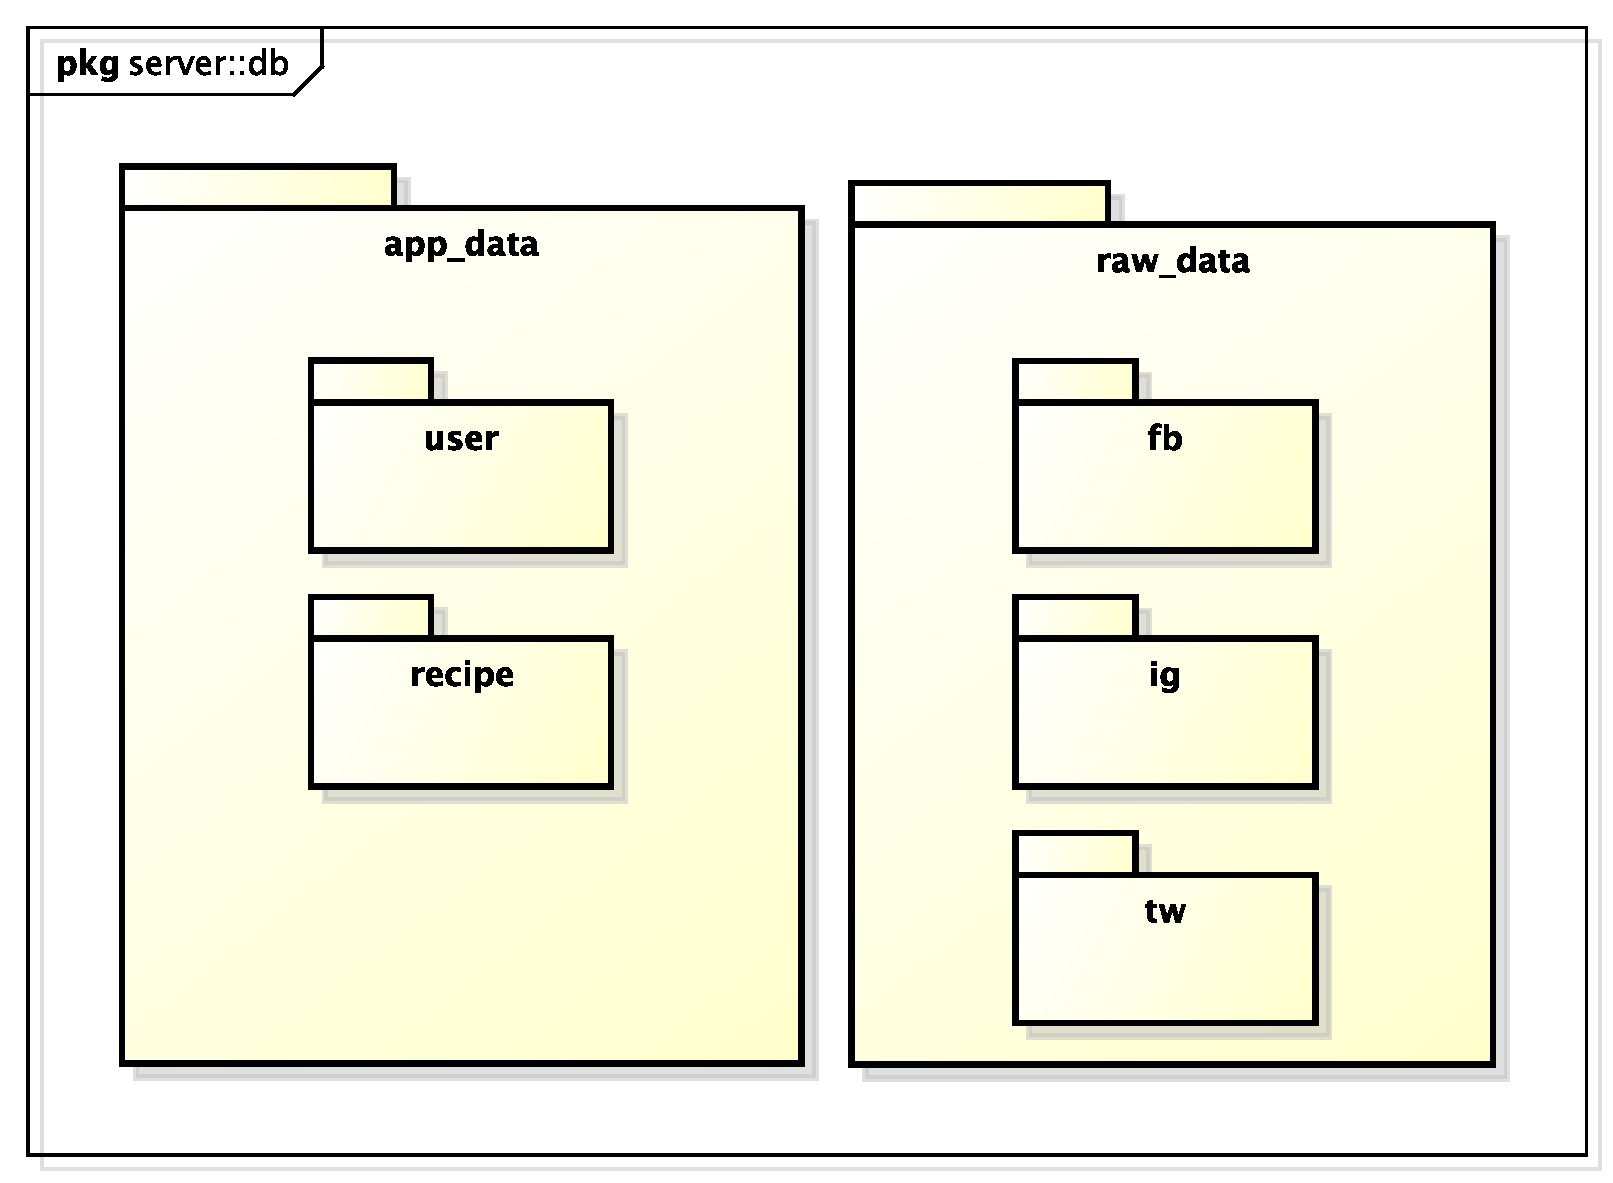
\includegraphics[scale=0.5]{./images/server/db.pdf}}
		\caption{Package - server::db}
	\end{figure}
	\begin{itemize}
		\item \textbf{Descrizione}: è il package che contiene le componenti che gestiscono e mantengono coerente la base di dati. Esse utilizzano standard proprietari Google per la loro implementazione. Sono suddivise in due package: uno atto a rappresentare il modello dei dati grezzi, l'altro dei parametri del software e degli utenti;
		\item \textbf{Padre}: server;
		\item \textbf{Package contenuti}:
			\begin{itemize}
				\item server::app\_data.
				\item server::raw\_data;
			\end{itemize}
	\end{itemize}

% subsubsection RAW_DATA
\subsubsection{server::db::raw\_data} % (fold)
\label{ssub:bdsm_app_server_raw_data}
	\begin{figure}[htbp]
		\centering
		\centerline{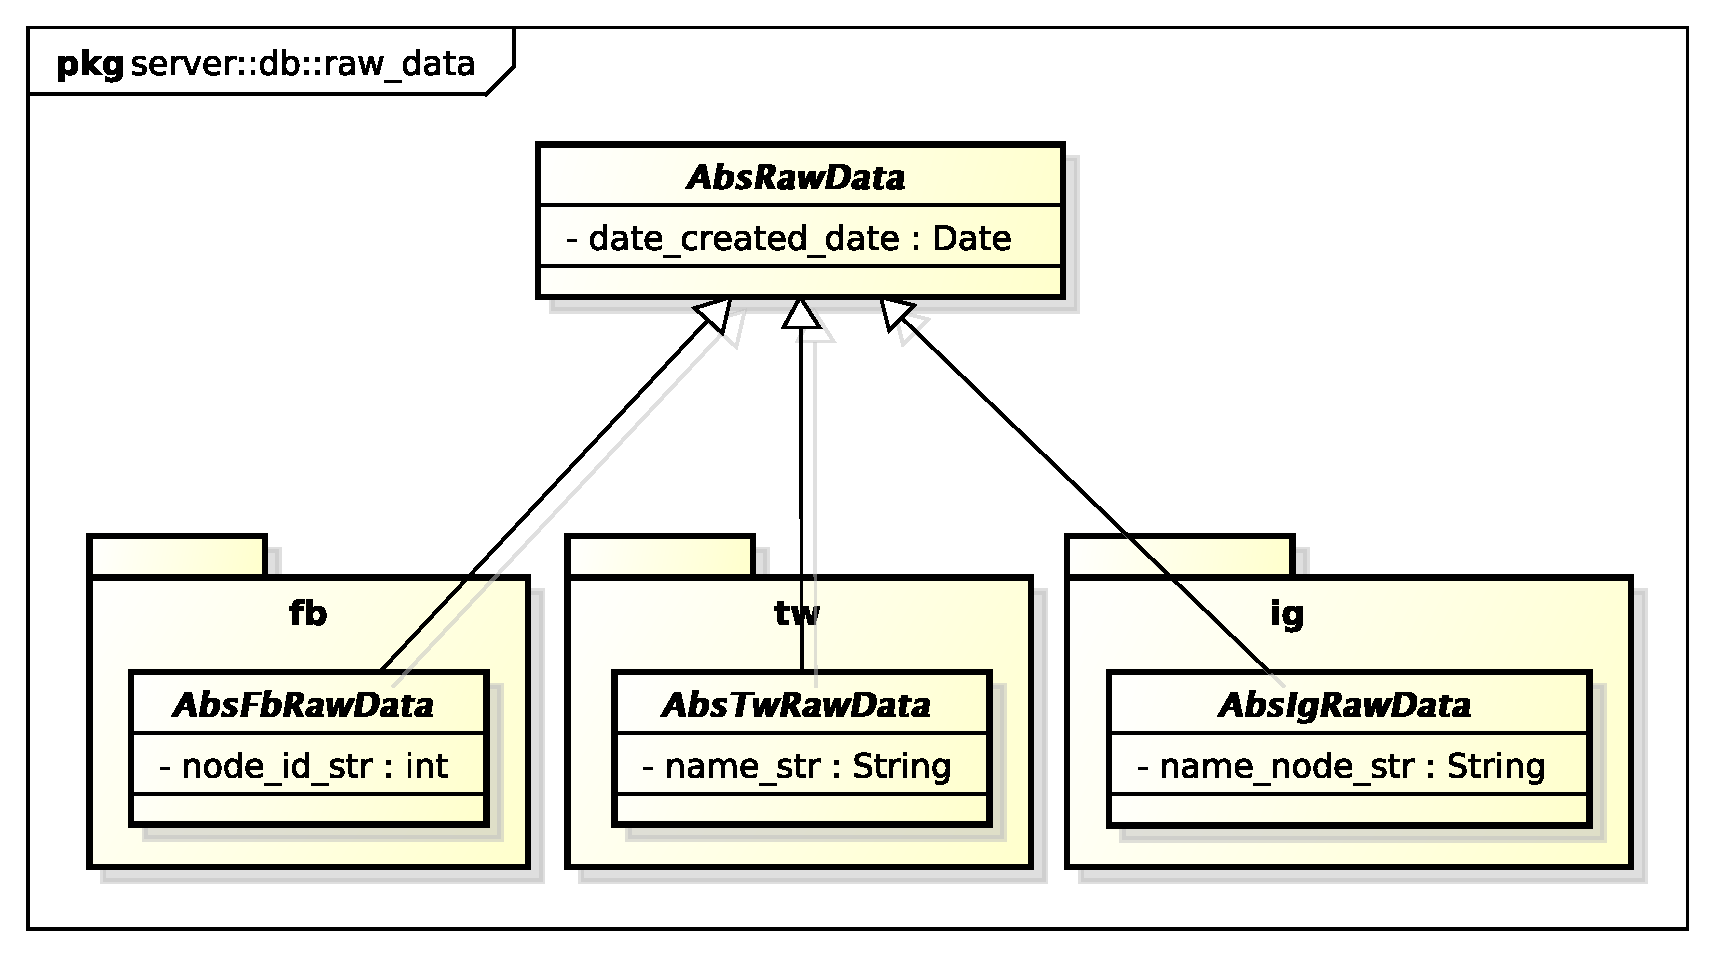
\includegraphics[scale=0.4]{./images/server/raw_data.pdf}}
		\caption{Package - server::db::raw\_data}
	\end{figure}
	\begin{itemize}
	\item \textbf{Descrizione}: package che definisce il modello dei dati grezzi ricavati dai vari social network;
		\item \textbf{Padre}: server::db;
		\item \textbf{Package contenuti}:
			\begin{itemize}
				\item server::db::raw\_data::fb
				\item server::db::raw\_data::tw
				\item server::db::raw\_data::ig
		\end{itemize}
	\end{itemize}

	\paragraph{Classi} % (fold)
		\subparagraph{server::db::raw\_data::AbsRawData} % (fold)
		\label{subp:bdsm_app_server_raw_data_absrawdata}
			\begin{itemize}
				\item \textbf{Descrizione}: classe astratta che definisce il modello di un dato grezzo;
				\item \textbf{Utilizzo}: la classe funge da padre per tutte le classi rappresentanti un dato grezzo;
				\item \textbf{Relazioni con altre classi}:
					\begin{itemize}
						\item server::db::raw\_data::fb::AbsFbRawData
						\item server::db::raw\_data::tw::AbsTwRawData
						\item server::db::raw\_data::ig::AbsIgRawData
						\item server::db::raw\_data::fb::RawFbPageTrend
						\item server::db::raw\_data::fb::RawFbEventTrend
						\item server::db::raw\_data::fb::RawFbPostTrendTrend
						\item server::db::raw\_data::tw::RawTwUserTrend
						\item server::db::raw\_data::tw::RawTwUserTweet
						\item server::db::raw\_data::ig::RawIgUserTrend
						\item server::db::raw\_data::ig::RawIgHashtagTrend
						\item server::db::raw\_data::ig::RawIgMedia
					\end{itemize}
				\item \textbf{Attributi}:
					\begin{itemize}
						\item \textcolor{forestgreen}{\texttt{+ date\_created\_date : Date}}
						\begin{description}
							\item \textbf{Descrizione}: data acquisizione dati grezzi
						\end{description}
					\end{itemize}
				\item \textbf{Metodi}: N/A
			\end{itemize}

		% subsubsection FACEBOOK
		\subsubsection{server::db::raw\_data::fb} % (fold)
		\label{ssub:bdsm_app_server_db_raw_data_fb}
		\begin{figure}[htbp]
			\centering
			\centerline{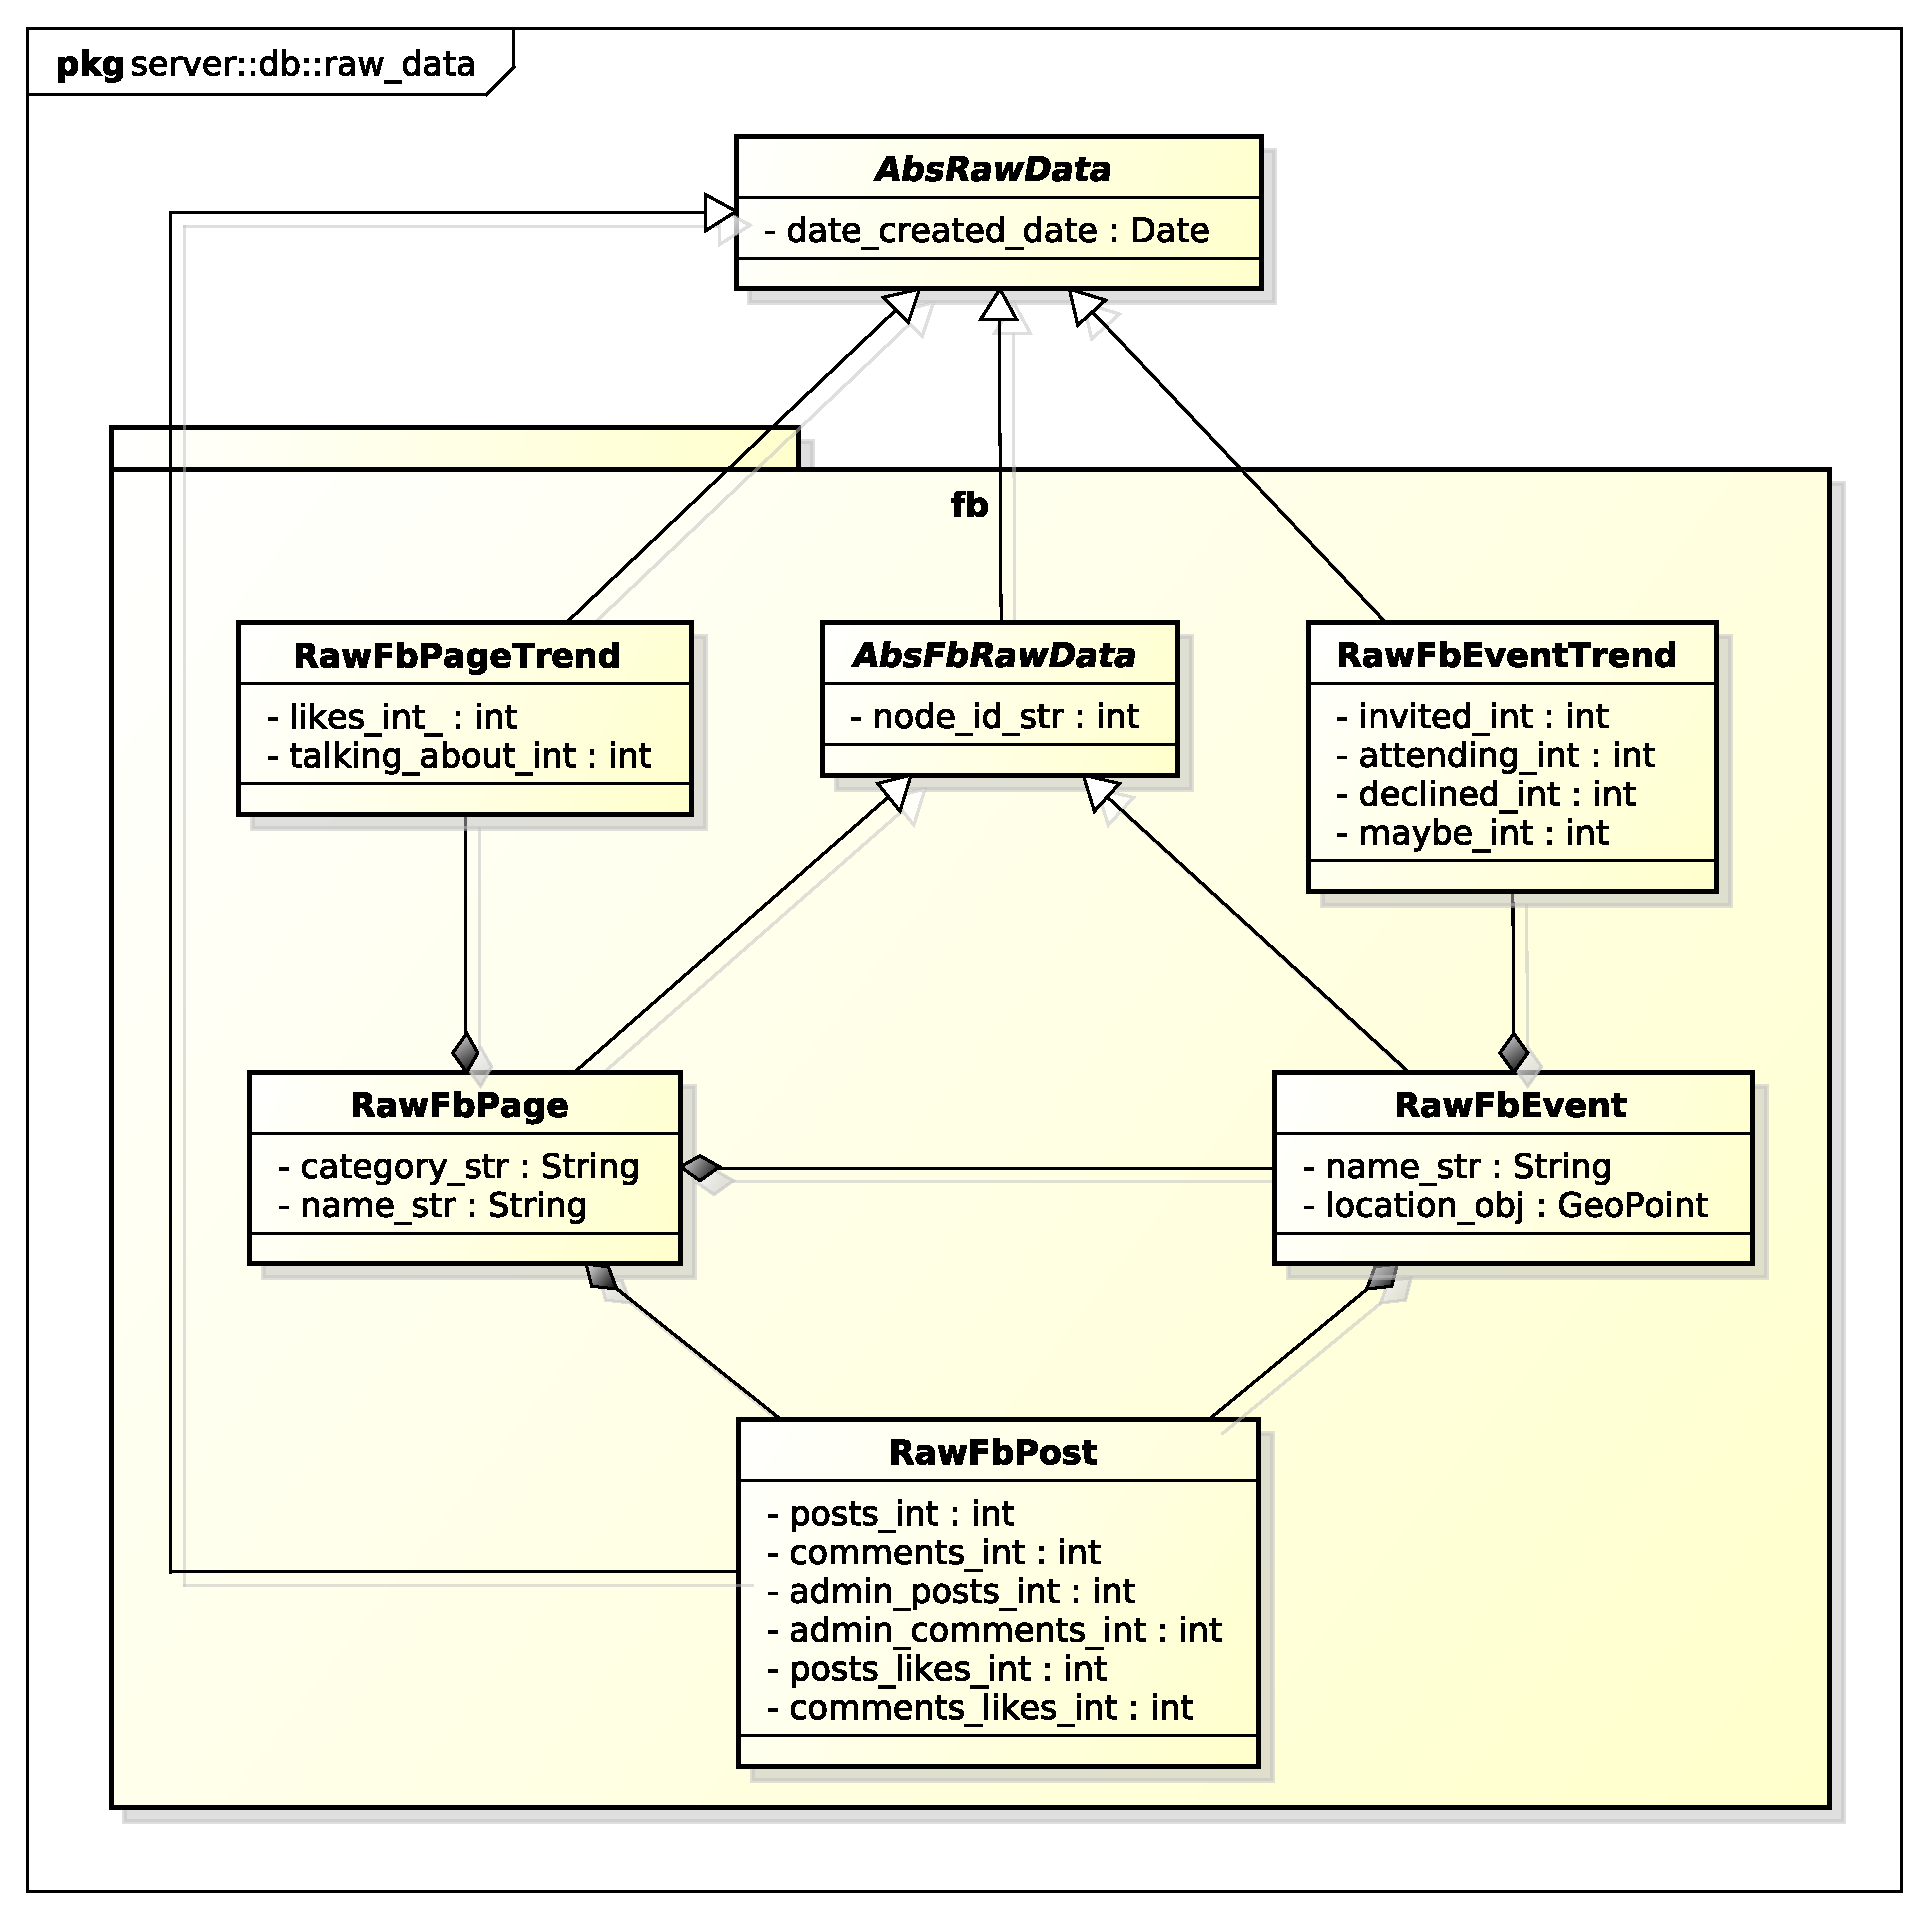
\includegraphics[scale=0.5]{./images/server/raw_data_fb.pdf}}
			\caption{Package - server::db::raw\_data::fb}
		\end{figure}
		\begin{itemize}
		  \item \textbf{Descrizione}:  è il package contenente le classi che definiscono i modelli dei dati grezzi relativi a Facebook;
		  \item \textbf{Padre}: server::db::raw\_data
		  \item \textbf{Interazione con altri componenti}:
		  	\begin{itemize}
		  		\item server::db
			\end{itemize}
		\end{itemize}
		% subsubsection

		\paragraph{Classi} % (fold)
			\subparagraph{server::db::raw\_data::fb::AbsFbRawData} % (fold)
			\label{subp:server_db_raw_data_fb_absfbrawdata}
				\begin{figure}[htbp]
					\centering
					\centerline{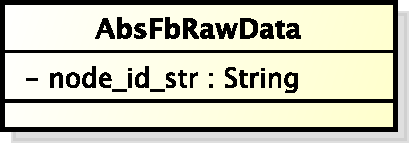
\includegraphics[scale=0.75]{./images/server/classes/db/abs_fb_raw_data.pdf}}
					\caption{Classe - server::db::raw\_data::fb::AbsFbRawData}
				\end{figure}
				\begin{itemize}
					\item \textbf{Descrizione}: classe astratta che definisce il modello dati grezzi relativi a Facebook;
					\item \textbf{Utilizzo}: la classe contiene l'id fornito dall'utente il quale permette di identificare univocamente la risorsa nel social media;
					\item \textbf{Classi ereditate}: server::db::raw\_data::AbsRawData
					\item \textbf{Attributi}:
					\begin{itemize}
						\item \textcolor{forestgreen}{\texttt{+ node\_id\_str : String}}
						\begin{description}
							\item \textbf{Descrizione}: codice identificativo evento o pagina Facebook
						\end{description}
					\end{itemize}
					\item \textbf{Metodi}: N/A
				\end{itemize}
			% subparagraph server_db_raw_data_fb_absfbrawdata [end]


			\subparagraph{server::db::raw\_data::fb::RawFbPage} % (fold)
			\label{subp:server_db_raw_data_fb_rawfbpage}			
				\begin{figure}[htbp]
					\centering
					\centerline{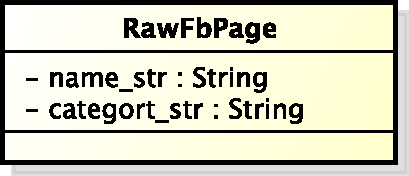
\includegraphics[scale=0.75]{./images/server/classes/db/raw_fb_page.pdf}}
					\caption{Classe - server::db::raw\_data::fb::RawFbPage}
				\end{figure}
				\begin{itemize}
					\item \textbf{Descrizione}: classe che rappresenta il modello di una pagina Facebook;
					\item \textbf{Utilizzo}: la classe fornisce metodi per memorizzare i dati statici di una pagina Facebook;
					\item \textbf{Classi ereditate}: server::db::raw\_data::AbsFbRawData
					\item \textbf{Relazioni con altre classi}:
						\begin{itemize}
							\item server::db::raw\_data::fb::RawFbEvent
							\item server::db::raw\_data::fb::RawFbPageTrend
							\item server::db::raw\_data::fb::RawFbPostTrend
						\end{itemize}
					\item \textbf{Attributi}:
					\begin{itemize}
						\item \textcolor{forestgreen}{\texttt{+ name\_str : String}}
						\begin{description}
							\item \textbf{Descrizione}: nome pagina Facebook
						\end{description}
						\item \textcolor{forestgreen}{\texttt{+ category\_str : String}}
						\begin{description}
							\item \textbf{Descrizione}: categoria pagina Facebook
						\end{description}
					\end{itemize}
					\item \textbf{Metodi}: N/A
				\end{itemize}
			% subparagraph server_db_raw_data_fb_rawfbpage [end]

			\subparagraph{server::db::raw\_data::fb::RawFbPageTrend} % (fold)
			\label{subp:server_db_raw_data_fb_rowfbpagetrend}
				\begin{figure}[htbp]
					\centering
					\centerline{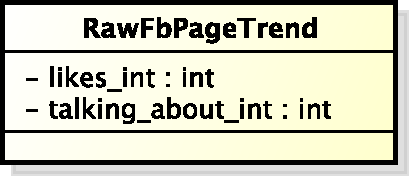
\includegraphics[scale=0.75]{./images/server/classes/db/raw_fb_page_trend.pdf}}
					\caption{Classe - server::db::raw\_data::fb::RawFbPageTrend}
				\end{figure}
				\begin{itemize}
					\item \textbf{Descrizione}: classe che rappresenta il modello del trend dei dati una pagina Facebook;
					\item \textbf{Utilizzo}: la classe viene utilizzata per memorizzare e il numero di like e di talking about di ogni singola pagina;
					\item \textbf{Classi ereditate}: server::db::raw\_data::AbsRawData
					\item \textbf{Attributi}:
					\begin{itemize}
						\item \textcolor{forestgreen}{\texttt{+ likes\_int : int}}
						\begin{description}
							\item \textbf{Descrizione}: numero likes di una determinata pagina Facebook
						\end{description}
						\item \textcolor{forestgreen}{\texttt{+ talking\_about\_int : int}}
						\begin{description}
							\item \textbf{Descrizione}: numero di talking about di una determinata pagina Facebook
						\end{description}
					\end{itemize}
					\item \textbf{Metodi}: N/A
				\end{itemize}
			% subparagraph server_db_raw_data_fb_rowfbpagetrend [end]


			\subparagraph{server::db::raw\_data::fb::RawFbEvent} % (fold)
			\label{subp:server_db_raw_data_fb_rawfbevent}
				\begin{figure}[htbp]
					\centering
					\centerline{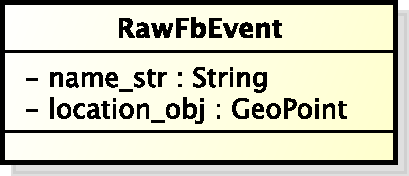
\includegraphics[scale=0.75]{./images/server/classes/db/raw_fb_event.pdf}}
					\caption{Classe - server::db::raw\_data::fb::RawFbEvent}
				\end{figure}
				\begin{itemize}
					\item \textbf{Descrizione}: classe che rappresenta il modello di un evento Facebook;
					\item \textbf{Utilizzo}: la classe fornisce metodi per memorizzare i dati statici di un evento Facebook;
					\item \textbf{Classi ereditate}: server::db::raw\_data::AbsFbRawData
					\item \textbf{Relazioni con altre classi}:
						\begin{itemize}
							\item server::db::raw\_data::fb::RawFbEventTrend
							\item server::db::raw\_data::fb::RawFbPostTrend
						\end{itemize}
					\item \textbf{Attributi}:
					\begin{itemize}
						\item \textcolor{forestgreen}{\texttt{+ name\_str : String}}
						\begin{description}
							\item \textbf{Descrizione}: nome evento Facebook
						\end{description}
						\item \textcolor{forestgreen}{\texttt{+ location\_obj : GeoPoint}}
						\begin{description}
							\item \textbf{Descrizione}: localizzazione tramite latitudine e longitudine pagina evento Facebook
						\end{description}
					\end{itemize}
					\item \textbf{Metodi}: N/A
				\end{itemize}
			% subparagraph server_db_raw_data_fb_rawfbevent [end]

			\subparagraph{server::db::raw\_data::fb::RawFbEventTrend} % (fold)
			\label{subp:server_db_raw_data_fb_rowfbeventtrend}
				\begin{figure}[htbp]
					\centering
					\centerline{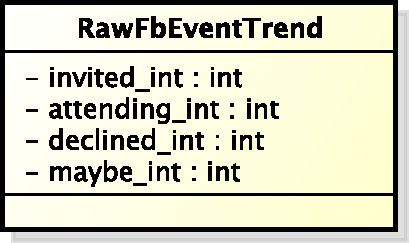
\includegraphics[scale=0.75]{./images/server/classes/db/raw_fb_event_trend.pdf}}
					\caption{Classe - server::db::raw\_data::fb::RawFbEventTrend}
				\end{figure}
				\begin{itemize}
					\item \textbf{Descrizione}: classe che rappresenta il modello del trend di un evento su Facebook;
					\item \textbf{Utilizzo}: la classe viene utilizzata per memorizzare il numero di utenti invitati, partecipanti e non di un evento;
					\item \textbf{Classi ereditate}: server::db::raw\_data::AbsRawData
					\item \textbf{Attributi}:
					\begin{itemize}
						\item \textcolor{forestgreen}{\texttt{+ invited\_int : int}}
						\begin{description}
							\item \textbf{Descrizione}: numero persone invitate evento Facebook
						\end{description}
						\item \textcolor{forestgreen}{\texttt{+ attending\_int : int}}
						\begin{description}
							\item \textbf{Descrizione}: numero persone partecipanti evento Facebook
						\end{description}
						\item \textcolor{forestgreen}{\texttt{+ declined\_int : int}}
						\begin{description}
							\item \textbf{Descrizione}: numero persone che hanno rifiutato la partecipazione evento Facebook
						\end{description}
						\item \textcolor{forestgreen}{\texttt{+ maybe\_int : int}}
						\begin{description}
							\item \textbf{Descrizione}: numero persone incerte se partecipare evento Facebook
						\end{description}
					\end{itemize}
					\item \textbf{Metodi}: N/A
				\end{itemize}
			% subparagraph server_db_raw_data_fb_rowfbeventtrend [end]


			\subparagraph{server::db::raw\_data::fb::RawFbPostTrend} % (fold)
			\label{subp:server_db_raw_data_fb_RawFbPostTrend}
				\begin{itemize}
					\item \textbf{Descrizione}: classe che rappresenta il modello del trend dei post di una pagina o di un evento su Facebook;
					\item \textbf{Utilizzo}: la classe fornisce metodi per sommare i dati statici sui post di Facebook;
					\item \textbf{Attributi}:
					\begin{itemize}
						\item \textcolor{forestgreen}{\texttt{+ posts\_int : int}}
						\begin{description}
							\item \textbf{Descrizione}: numero post utente
						\end{description}
						\item \textcolor{forestgreen}{\texttt{+ comments\_int : int}}
						\begin{description}
							\item \textbf{Descrizione}: numero commenti utente
						\end{description}
						\item \textcolor{forestgreen}{\texttt{+ admin\_posts\_int : int}}
						\begin{description}
							\item \textbf{Descrizione}: numero post admin
						\end{description}
						\item \textcolor{forestgreen}{\texttt{+ admin\_comments\_int : int}}
						\begin{description}
							\item \textbf{Descrizione}: numero commenti admin
						\end{description}
						\item \textcolor{forestgreen}{\texttt{+ posts\_like\_int : int}}
						\begin{description}
							\item \textbf{Descrizione}: numero like del post
						\end{description}
						\item \textcolor{forestgreen}{\texttt{+ comments\_like\_int : int}}
						\begin{description}
							\item \textbf{Descrizione}: numero like dei commenti
						\end{description}
					\end{itemize}
					\item \textbf{Metodi}: N/A
				\end{itemize}
			% subparagraph server_db_raw_data_fb_RawFbPostTrend [end]


		% subsubsection TWITTER
		\subsubsection{server::db::raw\_data::tw} % (fold)
		\label{ssub:bdsm_app_server_db_raw_data_tw}
		\begin{figure}[htbp]
			\centering
			\centerline{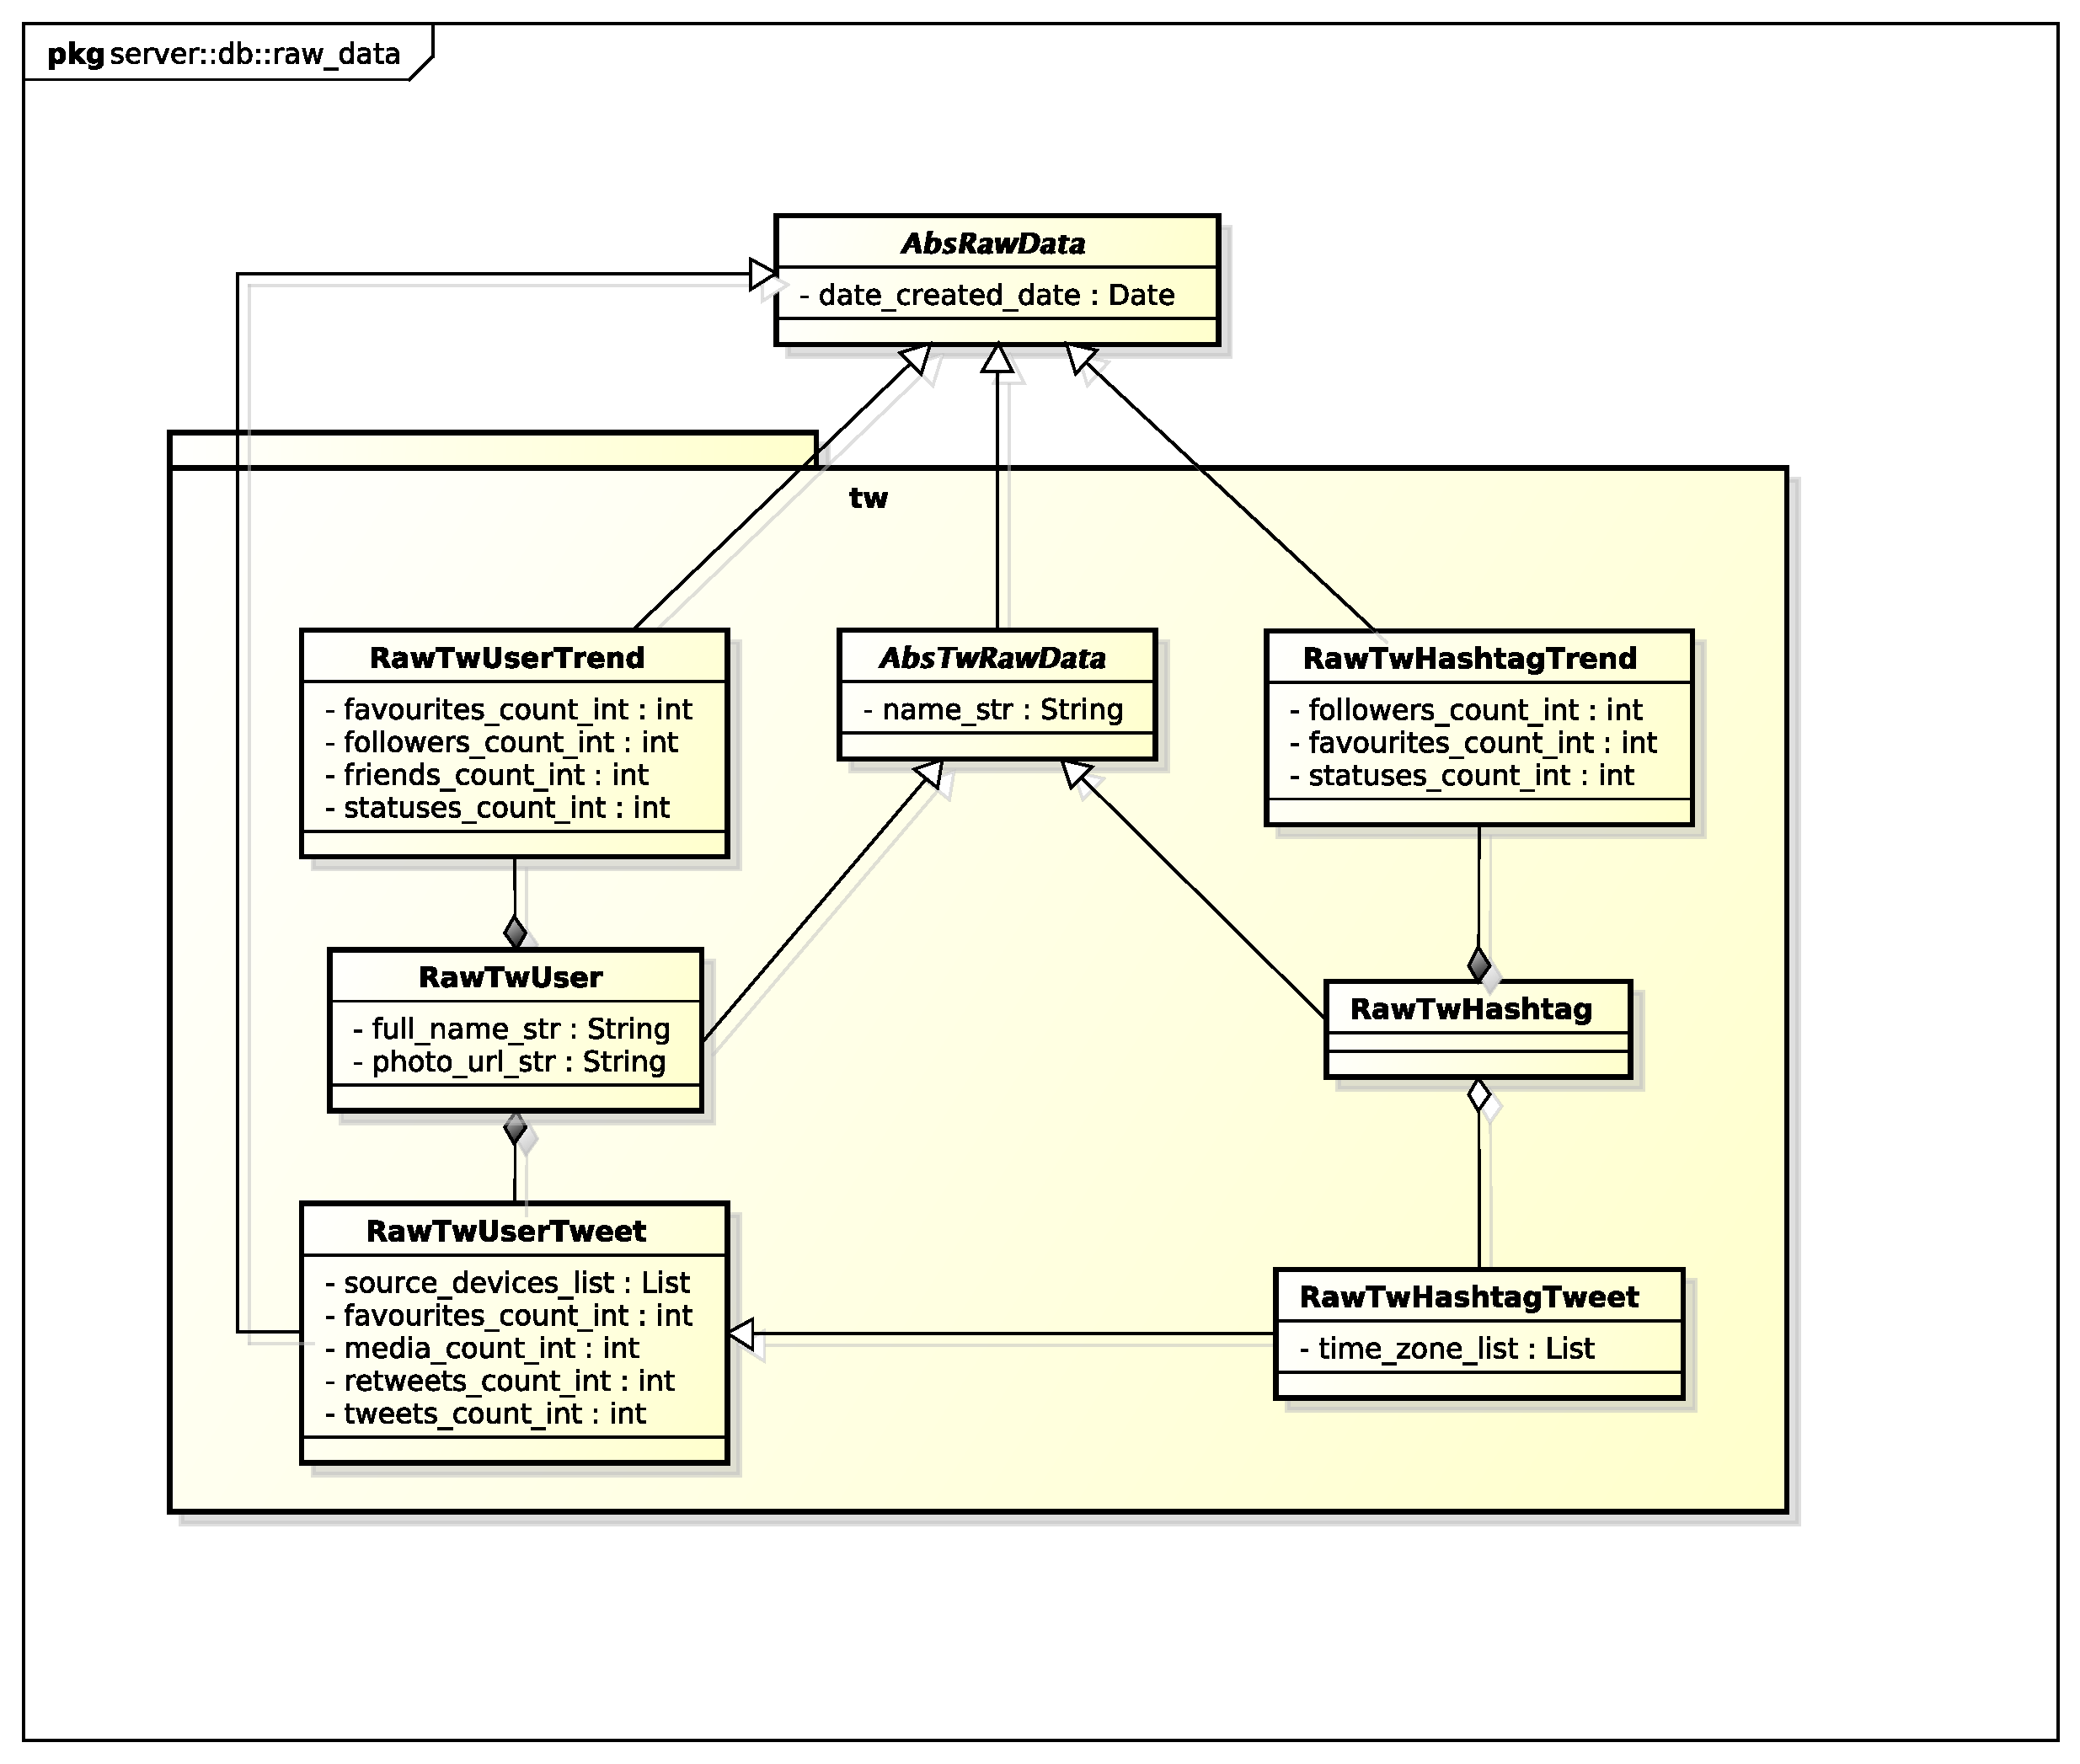
\includegraphics[scale=0.45]{./images/server/raw_data_tw.pdf}}
			\caption{Package - server::db::raw\_data::tw}
		\end{figure}

		\begin{itemize}
		  \item \textbf{Descrizione}: è il package contenente le classi che definiscono i modelli dei dati grezzi relativi a Twitter;
		  \item \textbf{Padre}: server::db::raw\_data
		  \item \textbf{Interazione con altri componenti}:
		  	\begin{itemize}
		  		\item server::db
			\end{itemize}
		\end{itemize}
		% subsubsection

		\paragraph{Classi} % (fold)


		\subparagraph{server::db::raw\_data::tw::AbsTwRawData} % (fold)
		\label{subp:server_db_raw_data_tw_abstwrawdata}
			\begin{figure}[htbp]
				\centering
				\centerline{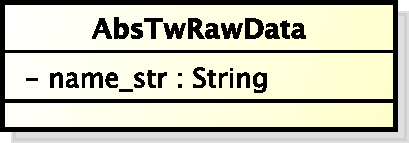
\includegraphics[scale=0.75]{./images/server/classes/db/abs_tw_raw_data.pdf}}
				\caption{Classe - server::db::raw\_data::tw::AbsTwRawData}
			\end{figure}
			\begin{itemize}
				\item \textbf{Descrizione}: classe astratta che definisce il modello dati grezzi relativi a Twitter;
				\item \textbf{Utilizzo}: la classe contiene l'id fornito dall'utente il quale permette di identificare univocamente la risorsa nel social media;
				\item \textbf{Classi ereditate}: server::db::raw\_data::AbsRawData
				\item \textbf{Attributi}:
					\begin{itemize}
						\item \textcolor{forestgreen}{\texttt{+ name\_str : String}}
						\begin{description}
							\item \textbf{Descrizione}: nome identificativo pagina o hashtag
						\end{description}
					\end{itemize}
				\item \textbf{Metodi}: N/A
			\end{itemize}
		% subparagraph server_db_raw_data_tw_abstwrawdata [end]


		\subparagraph{server::db::raw\_data::tw::RawTwUser} % (fold)
		\label{subp:server_db_raw_data_tw_rawtwuser}
			\begin{figure}[htbp]
				\centering
				\centerline{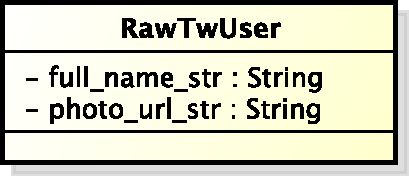
\includegraphics[scale=0.75]{./images/server/classes/db/raw_tw_user.pdf}}
				\caption{Classe - server::db::raw\_data::tw::RawTwUser}
			\end{figure}
			\begin{itemize}
				\item \textbf{Descrizione}: classe che definisce il modello dei dati di un utente Twitter;
				\item \textbf{Utilizzo}: la classe viene utilizzata per fornire una descrizione completa dell'utente Twitter. Vengono forniti metodi automatici per il conteggio dei parametri che verranno utilizzati per seguire un trend;;
				\item \textbf{Classi ereditate}: server::db::raw\_data::AbsTwRawData
				\item \textbf{Relazioni con altre classi}:
					\begin{itemize}
						\item server::db::raw\_data::tw::RawTwUserTrend
						\item server::db::raw\_data::tw::RawTwUserTweet
					\end{itemize}
				\item \textbf{Attributi}:
					\begin{itemize}
						\item \textcolor{forestgreen}{\texttt{+ full\_name\_str : String}}
						\begin{description}
							\item \textbf{Descrizione}: nome completo del profilo utente
						\end{description}
						\item \textcolor{forestgreen}{\texttt{+ photo\_url\_str : String}}
						\begin{description}
							\item \textbf{Descrizione}: indirizzo url foto profilo utente
						\end{description}
					\end{itemize}
				\item \textbf{Metodi}: N/A
			\end{itemize}
		% subparagraph server_db_raw_data_tw_rawtwuser [end]


		\subparagraph{server::db::raw\_data::tw::RawTwUserTrend} % (fold)
		\label{subp:server_db_raw_data_tw_rawigusertrend}
			\begin{figure}[htbp]
				\centering
				\centerline{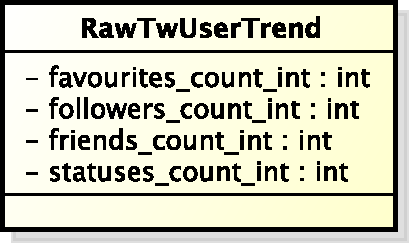
\includegraphics[scale=0.75]{./images/server/classes/db/raw_tw_user_trend.pdf}}
				\caption{Classe - server::db::raw\_data::tw::RawTwUserTrend}
			\end{figure}
			\begin{itemize}
				\item \textbf{Descrizione}: classe che definisce il modello dei dati del trend di un utente Twitter;
				\item \textbf{Utilizzo}: la classe viene utilizzata per memorizzare il numero di favoriti, di followers, di friends e statuses di una determinata persona;
				\item \textbf{Classi ereditate}: server::db::raw\_data::AbsTwRawData
				\item \textbf{Attributi}:
					\begin{itemize}
						\item \textcolor{forestgreen}{\texttt{+ favourites\_count\_int : int}}
						\begin{description}
							\item \textbf{Descrizione}: numero di favoriti utente Twitter
						\end{description}
						\item \textcolor{forestgreen}{\texttt{+ followers\_count\_int : int}}
						\begin{description}
							\item \textbf{Descrizione}: numero di followers utente Twitter
						\end{description}
						\item \textcolor{forestgreen}{\texttt{+ friends\_count\_int : int}}
						\begin{description}
							\item \textbf{Descrizione}: numero di amici utente Twitter
						\end{description}
						\item \textcolor{forestgreen}{\texttt{+ tweets\_count\_int : int}}
						\begin{description}
							\item \textbf{Descrizione}: numero di tweets utente Twitter
						\end{description}
					\end{itemize}
				\item \textbf{Metodi}: N/A
			\end{itemize}
		% subparagraph server_db_raw_data_tw_rawigusertrend [end]


		\subparagraph{server::db::raw\_data::tw::RawTwUserTweet} % (fold)
		\label{subp:server_db_raw_data_tw_rawtwusertweet}
			\begin{figure}[htbp]
				\centering
				\centerline{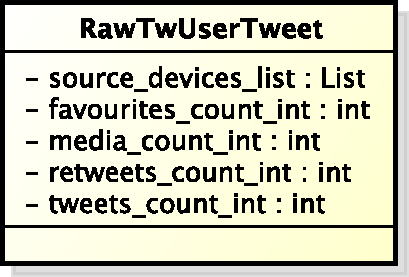
\includegraphics[scale=0.75]{./images/server/classes/db/raw_tw_user_tweet.pdf}}
				\caption{Classe - server::db::raw\_data::tw::RawTwUserTweet}
			\end{figure}
			\begin{itemize}
				\item \textbf{Descrizione}: classe che definisce il modello dei dati del trend dei tweet relativi ad un utente Twitter;
				\item \textbf{Utilizzo}: la classe viene utilizzata per fornire una descrizione dettagliata di un tweet creato da un utente specifico su Twitter;
				\item \textbf{Classi ereditate}: server::db::raw\_data::AbsRawData
				\item \textbf{Attributi}:
					\begin{itemize}
						\item \textcolor{forestgreen}{\texttt{+ source\_devices\_list : List}}
						\begin{description}
							\item \textbf{Descrizione}: lista composta da quantità e tipo dispositivi utilizzati per pubblicazione tweet
						\end{description}
						\item \textcolor{forestgreen}{\texttt{+ favourites\_count\_int : int}}
						\begin{description}
							\item \textbf{Descrizione}: somma della quantità di favoriti dei tweets
						\end{description}
						\item \textcolor{forestgreen}{\texttt{+ retweets\_count\_int : int}}
						\begin{description}
							\item \textbf{Descrizione}: somma della quantità di retweets dei tweets
						\end{description}
					\end{itemize}
				\item \textbf{Metodi}: N/A
			\end{itemize}
		% subparagraph server_db_raw_data_tw_rawtwusertweet [end]


		\subparagraph{server::db::raw\_data::tw::RawTwHashtag} % (fold)
		\label{subp:server_db_raw_data_tw_rawtwhashtag}
			\begin{itemize}
				\item \textbf{Descrizione}: classe che definisce il modello dei dati di un hashtag su Twitter;
				\item \textbf{Utilizzo}: la classe viene utilizzata per fornire una descrizione minimale di un hashtag su Twitter. Vengono forniti metodi automatici per il conteggio dei parametri che verranno utilizzati per seguire un trend;
				\item \textbf{Classi ereditate}: server::db::raw\_data::AbsTwRawData
				\item \textbf{Relazioni con altre classi}:
					\begin{itemize}
						\item server::db::raw\_data::tw::RawTwHashtagTweet
					\end{itemize}
				\item \textbf{Attributi}: N/A
				\item \textbf{Metodi}: N/A
			\end{itemize}
		% subparagraph server_db_raw_data_tw_rawtwhashtag [end]


		\subparagraph{server::db::raw\_data::tw::RawTwHashtagTweet} % (fold)
		\label{subp:server_db_raw_data_tw_rawtwhashtagtweet}
			\begin{figure}[htbp]
				\centering
				\centerline{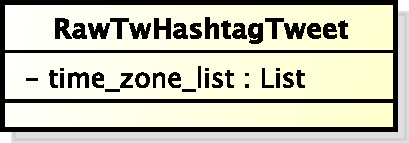
\includegraphics[scale=0.75]{./images/server/classes/db/raw_tw_hashtag_tweet.pdf}}
				\caption{Classe - server::db::raw\_data::tw::RawTwHashtagTweet}
			\end{figure}
			\begin{itemize}
				\item \textbf{Descrizione}: classe che definisce il modello dei dati del trend dei tweet relativi ad un hashtag Twitter;
				\item \textbf{Utilizzo}: la classe viene utilizzata per fornire una descrizione della locazione spaziale di un tweet relativo all'hashtag su Twitter;
				\item \textbf{Classi ereditate}: server::db::raw\_data::RawTwUserTweet
				\item \textbf{Attributi}:
					\begin{itemize}
						\item \textcolor{forestgreen}{\texttt{+ time\_zone\_list : List}}
						\begin{description}
							\item \textbf{Descrizione}: lista composta da quantità è timezone ricavati dai tweets contenenti il determinato hashtag
						\end{description}
						\item \textcolor{forestgreen}{\texttt{+ tweets\_count\_int : int}}
						\begin{description}
							\item \textbf{Descrizione}: somma dei tweets contenenti un determinato hashtag
						\end{description}
					\end{itemize}
				\item \textbf{Metodi}: N/A
			\end{itemize}
		% subparagraph server_db_raw_data_tw_rawtwhashtagtweet [end]


		% subsubsection INSTAGRAM
		\subsubsection{server::db::raw\_data::ig} % (fold)
		\label{ssub:bdsm_app_server_db_raw_data_ig}
		\begin{figure}[htbp]
			\centering
			\centerline{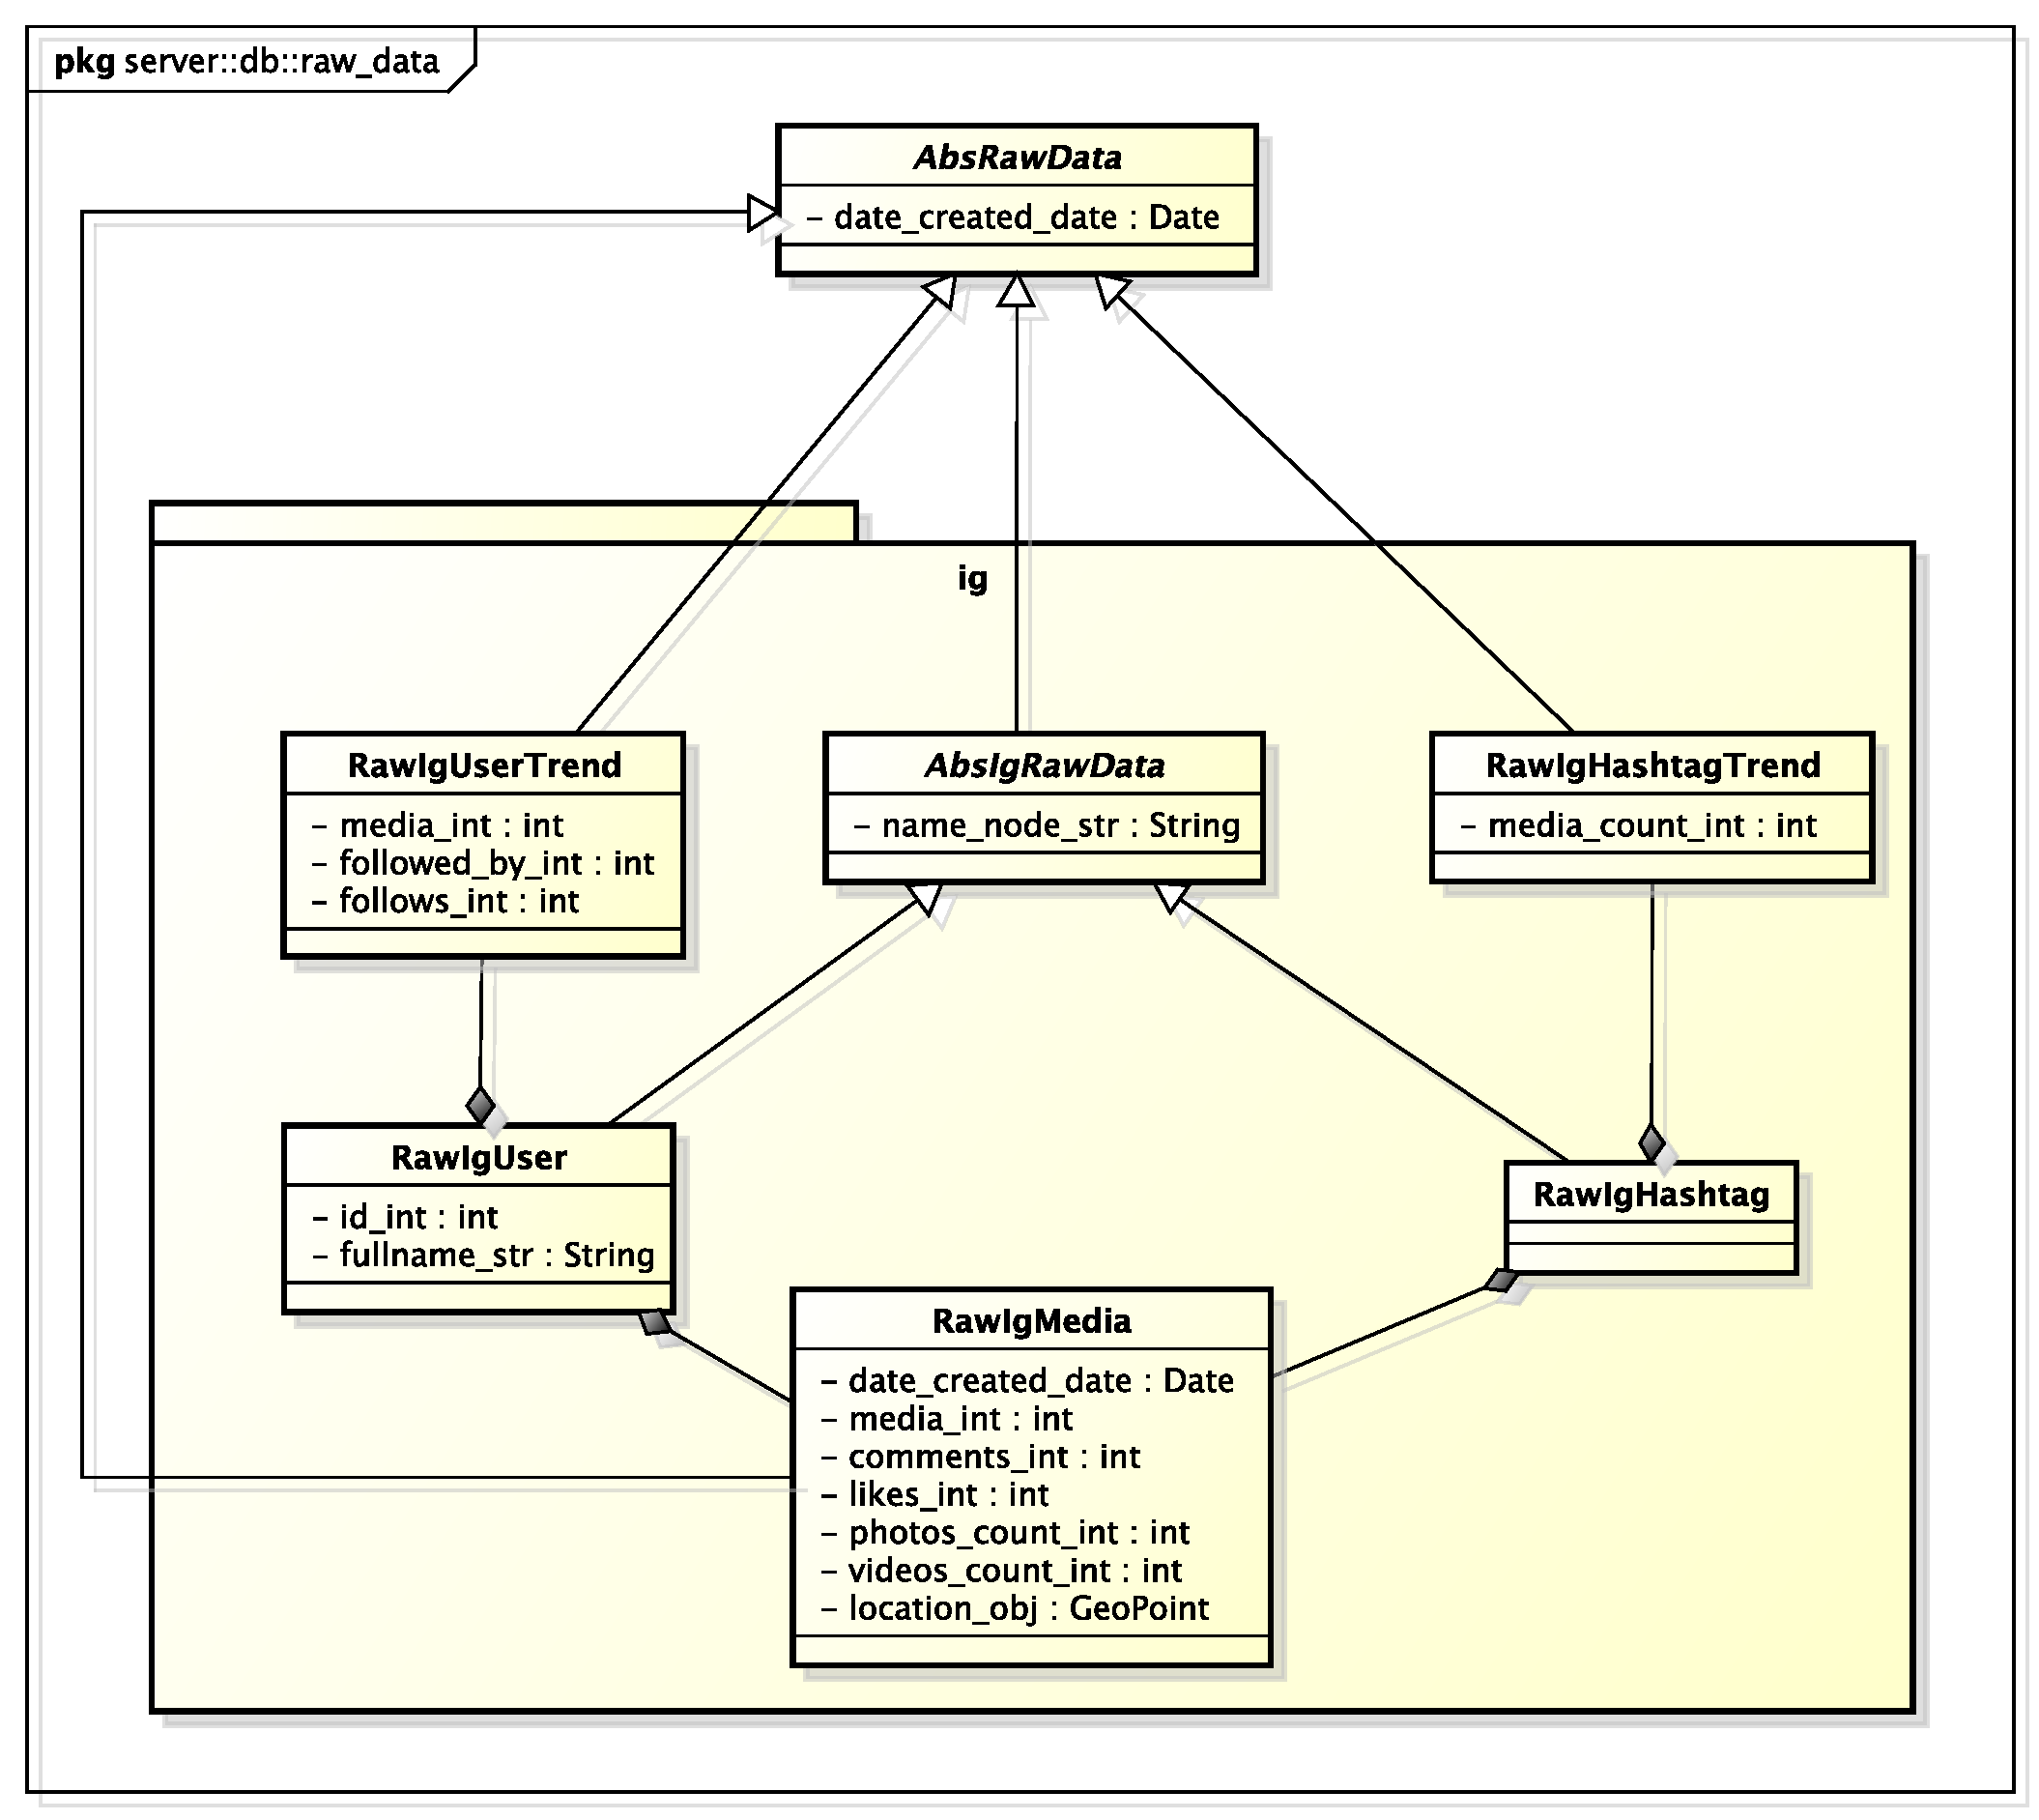
\includegraphics[scale=0.5]{./images/server/raw_data_ig.pdf}}
			\caption{Package - server::db::raw\_data::ig}
		\end{figure}

		\begin{itemize}
		  \item \textbf{Descrizione}: è il package contenente le classi che definiscono i modelli dei dati grezzi relativi a Instagram;
		  \item \textbf{Padre}: server::db::raw\_data
		  \item \textbf{Interazione con altri componenti}:
		  	\begin{itemize}
		  		\item server::db
				\end{itemize}
		\end{itemize}
		% subsubsection

		\paragraph{Classi} % (fold)


		\subparagraph{server::db::raw\_data::ig::AbsIgRawData} % (fold)
		\label{subp:server_db_raw_data_ig_absigrawdata}
			\begin{figure}[htbp]
				\centering
				\centerline{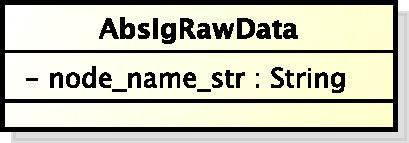
\includegraphics[scale=0.75]{./images/server/classes/db/abs_ig_raw_data.pdf}}
				\caption{Classe - server::db::raw\_data::ig::AbsIgRawData}
			\end{figure}
			\begin{itemize}
				\item \textbf{Descrizione}: classe astratta che definisce il modello dei dati grezzi relativi ad Instagram;
				\item \textbf{Utilizzo}: la classe contiene l'id fornito dall'utente il quale permette di identificare univocamente la risorsa nel social media;
				\item \textbf{Classi ereditate}: server::db::raw\_data::AbsRawData
				\item \textbf{Attributi}:
					\begin{itemize}
						\item \textcolor{forestgreen}{\texttt{+ node\_name\_str : String}}
						\begin{description}
							\item \textbf{Descrizione}: nome identificativo pagina o hashtag
						\end{description}
					\end{itemize}
				\item \textbf{Metodi}: N/A
			\end{itemize}
		% subparagraph server_db_raw_data_ig_absigrawdata [end]


		\subparagraph{server::db::raw\_data::ig::RawIgUser} % (fold)
		\label{subp:server_db_raw_data_ig_rawiguser}
			\begin{figure}[htbp]
				\centering
				\centerline{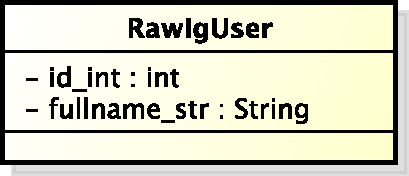
\includegraphics[scale=0.75]{./images/server/classes/db/raw_ig_user.pdf}}
				\caption{Classe - server::db::raw\_data::ig::RawIgUser}
			\end{figure}
			\begin{itemize}
				\item \textbf{Descrizione}: classe che definisce il modello dei dati di un utente Instagram;
				\item \textbf{Utilizzo}:  la classe viene utilizzata per memorizzare le i dettagli di un utente Instagram;
				\item \textbf{Classi ereditate}: server::db::raw\_data::AbsIgRawData
				\item \textbf{Relazioni con altre classi}:
					\begin{itemize}
						\item server::db::raw\_data::ig::RawIgUserTrend
						\item server::db::raw\_data::ig::RawIgMedia
					\end{itemize}
				\item \textbf{Attributi}:
					\begin{itemize}
						\item \textcolor{forestgreen}{\texttt{+ id\_int : int}}
						\begin{description}
							\item \textbf{Descrizione}: numero identificativo utente Instagram
						\end{description}
						\item \textcolor{forestgreen}{\texttt{+ fullname\_str : String}}
						\begin{description}
							\item \textbf{Descrizione}: nome completo del profilo utente Instagram
						\end{description}
					\end{itemize}
				\item \textbf{Metodi}: N/A
			\end{itemize}
		% subparagraph server_db_raw_data_ig_rawiguser [end]


		\subparagraph{server::db::raw\_data::ig::RawIgUserTrend} % (fold)
		\label{subp:server_db_raw_data_ig_rawigusertrend}
			\begin{figure}[htbp]
				\centering
				\centerline{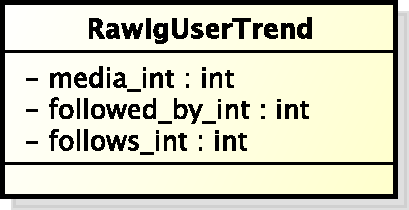
\includegraphics[scale=0.75]{./images/server/classes/db/raw_ig_user_trend.pdf}}
				\caption{Classe - server::db::raw\_data::ig::RawIgUserTrend}
			\end{figure}
			\begin{itemize}
				\item \textbf{Descrizione}: classe che definisce il modello dei dati del trend di un utente Instagram;
				\item \textbf{Utilizzo}: la classe viene utilizzata per memorizzare il numero di media, di followed e follows di una determinata persona;
				\item \textbf{Classi ereditate}: server::db::raw\_data::AbsRawData
				\item \textbf{Attributi}:
					\begin{itemize}
						\item \textcolor{forestgreen}{\texttt{+ media\_int : int}}
						\begin{description}
							\item \textbf{Descrizione}: numero di media caricati dall'utente su Instagram
						\end{description}
						\item \textcolor{forestgreen}{\texttt{+ followed\_by\_int : int}}
						\begin{description}
							\item \textbf{Descrizione}: numero di followed dell'utente
						\end{description}
						\item \textcolor{forestgreen}{\texttt{+ follows\_int : int}}
						\begin{description}
							\item \textbf{Descrizione}: numero di follows che segue l'utente
						\end{description}
					\end{itemize}
				\item \textbf{Metodi}: N/A
			\end{itemize}
		% subparagraph server_db_raw_data_ig_rawigusertrend [end]


		\subparagraph{server::db::raw\_data::ig::RawIgHashtag} % (fold)
		\label{subp:server_db_raw_data_ig_rawighashtag}
			\begin{itemize}
				\item \textbf{Descrizione}: classe che definisce il modello dei dati di un hashtag Instagram;
				\item \textbf{Utilizzo}: la classe viene utilizzata per fornire una descrizione minimale dell'hashtag su Instagram;
				\item \textbf{Classi ereditate}: server::db::raw\_data::AbsIgRawData
				\item \textbf{Relazioni con altre classi}:
					\begin{itemize}
						\item server::db::raw\_data::ig::RawIgHashtagTrend
						\item server::db::raw\_data::ig::RawIgMedia
					\end{itemize}
				\item \textbf{Attributi}: N/A
				\item \textbf{Metodi}: N/A
			\end{itemize}
		% subparagraph server_db_raw_data_ig_rawighashtag [end]


		\subparagraph{server::db::raw\_data::ig::RawIgHashtagTrend} % (fold)
		\label{subp:server_db_raw_data_ig_rawighashtagtrend}
			\begin{figure}[htbp]
				\centering
				\centerline{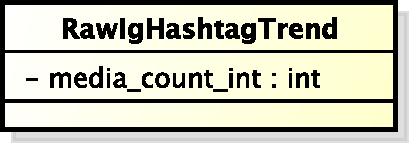
\includegraphics[scale=0.75]{./images/server/classes/db/raw_ig_hashtag_trend.pdf}}
				\caption{Classe - server::db::raw\_data::ig::RawIgHashtagTrend}
			\end{figure}
			\begin{itemize}
				\item \textbf{Descrizione}: classe che definisce il modello dei dati del trend di un hastag Instagram;
				\item \textbf{Utilizzo}: la classe viene utilizzata per memorizzare il numero di media caricati di un determinato hashtag;
				\item \textbf{Classi ereditate}: server::db::raw\_data::AbsRawData
				\item \textbf{Attributi}:
					\begin{itemize}
						\item \textcolor{forestgreen}{\texttt{+ media\_count\_int : int}}
						\begin{description}
							\item \textbf{Descrizione}: numero totale di media caricati dato un hashtag su Instagram
						\end{description}
					\end{itemize}
				\item \textbf{Metodi}: N/A
			\end{itemize}
		% subparagraph server_db_raw_data_ig_rawighashtagtrend [end]


		\subparagraph{server::db::raw\_data::ig::RawIgMedia} % (fold)
		\label{subp:server_db_raw_data_ig_rawigmedia}
			\begin{figure}[htbp]
				\centering
				\centerline{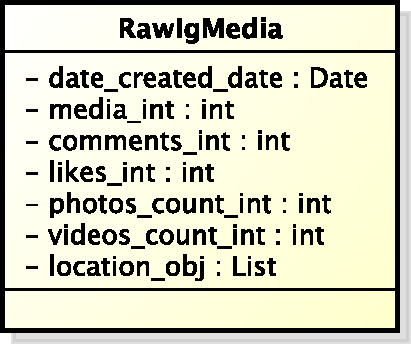
\includegraphics[scale=0.75]{./images/server/classes/db/raw_ig_media.pdf}}
				\caption{Classe - server::db::raw\_data::ig::RawIgMedia}
			\end{figure}
			\begin{itemize}
				\item \textbf{Descrizione}: classe che definisce il modello dei dati di un media realtivo ad Instagram;
				\item \textbf{Utilizzo}: la classe viene utilizzata per fornire una descrizione dettagliata di un media caricato da un utente specifico su Instagram. Vengono forniti metodi automatici per il conteggio dei parametri che verranno utilizzati per seguire un trend;
				\item \textbf{Classi ereditate}: server::db::raw\_data::AbsRawData
				\item \textbf{Attributi}:
					\begin{itemize}
						\item \textcolor{forestgreen}{\texttt{+ media\_int : int}}
						\begin{description}
							\item \textbf{Descrizione}: numero identificativo media su Instagram
						\end{description}
						\item \textcolor{forestgreen}{\texttt{+ comments\_int : int}}
						\begin{description}
							\item \textbf{Descrizione}: numero di commenti del media
						\end{description}
						\item \textcolor{forestgreen}{\texttt{+ likes\_int : int}}
						\begin{description}
							\item \textbf{Descrizione}: numero di like del media
						\end{description}
						\item \textcolor{forestgreen}{\texttt{+ photos\_count\_int : int}}
						\begin{description}
							\item \textbf{Descrizione}: numero di foto del media
						\end{description}
						\item \textcolor{forestgreen}{\texttt{+ videos\_count\_int : int}}
						\begin{description}
							\item \textbf{Descrizione}: numero di video del media
						\end{description}
						\item \textcolor{forestgreen}{\texttt{+ location\_obj : GeoPoint}}
						\begin{description}
							\item \textbf{Descrizione}: localizzazione tramite latitudine e longitudine di un media su Instagram
						\end{description}
					\end{itemize}
				\item \textbf{Metodi}: N/A
			\end{itemize}
		% subparagraph server_db_raw_data_ig_rawigmedia [end]

\subsubsection{server::db::app\_data} % (fold)
\label{ssub:bdsm_app_server_app_data}


	\begin{figure}[htbp]
		\centering
		\centerline{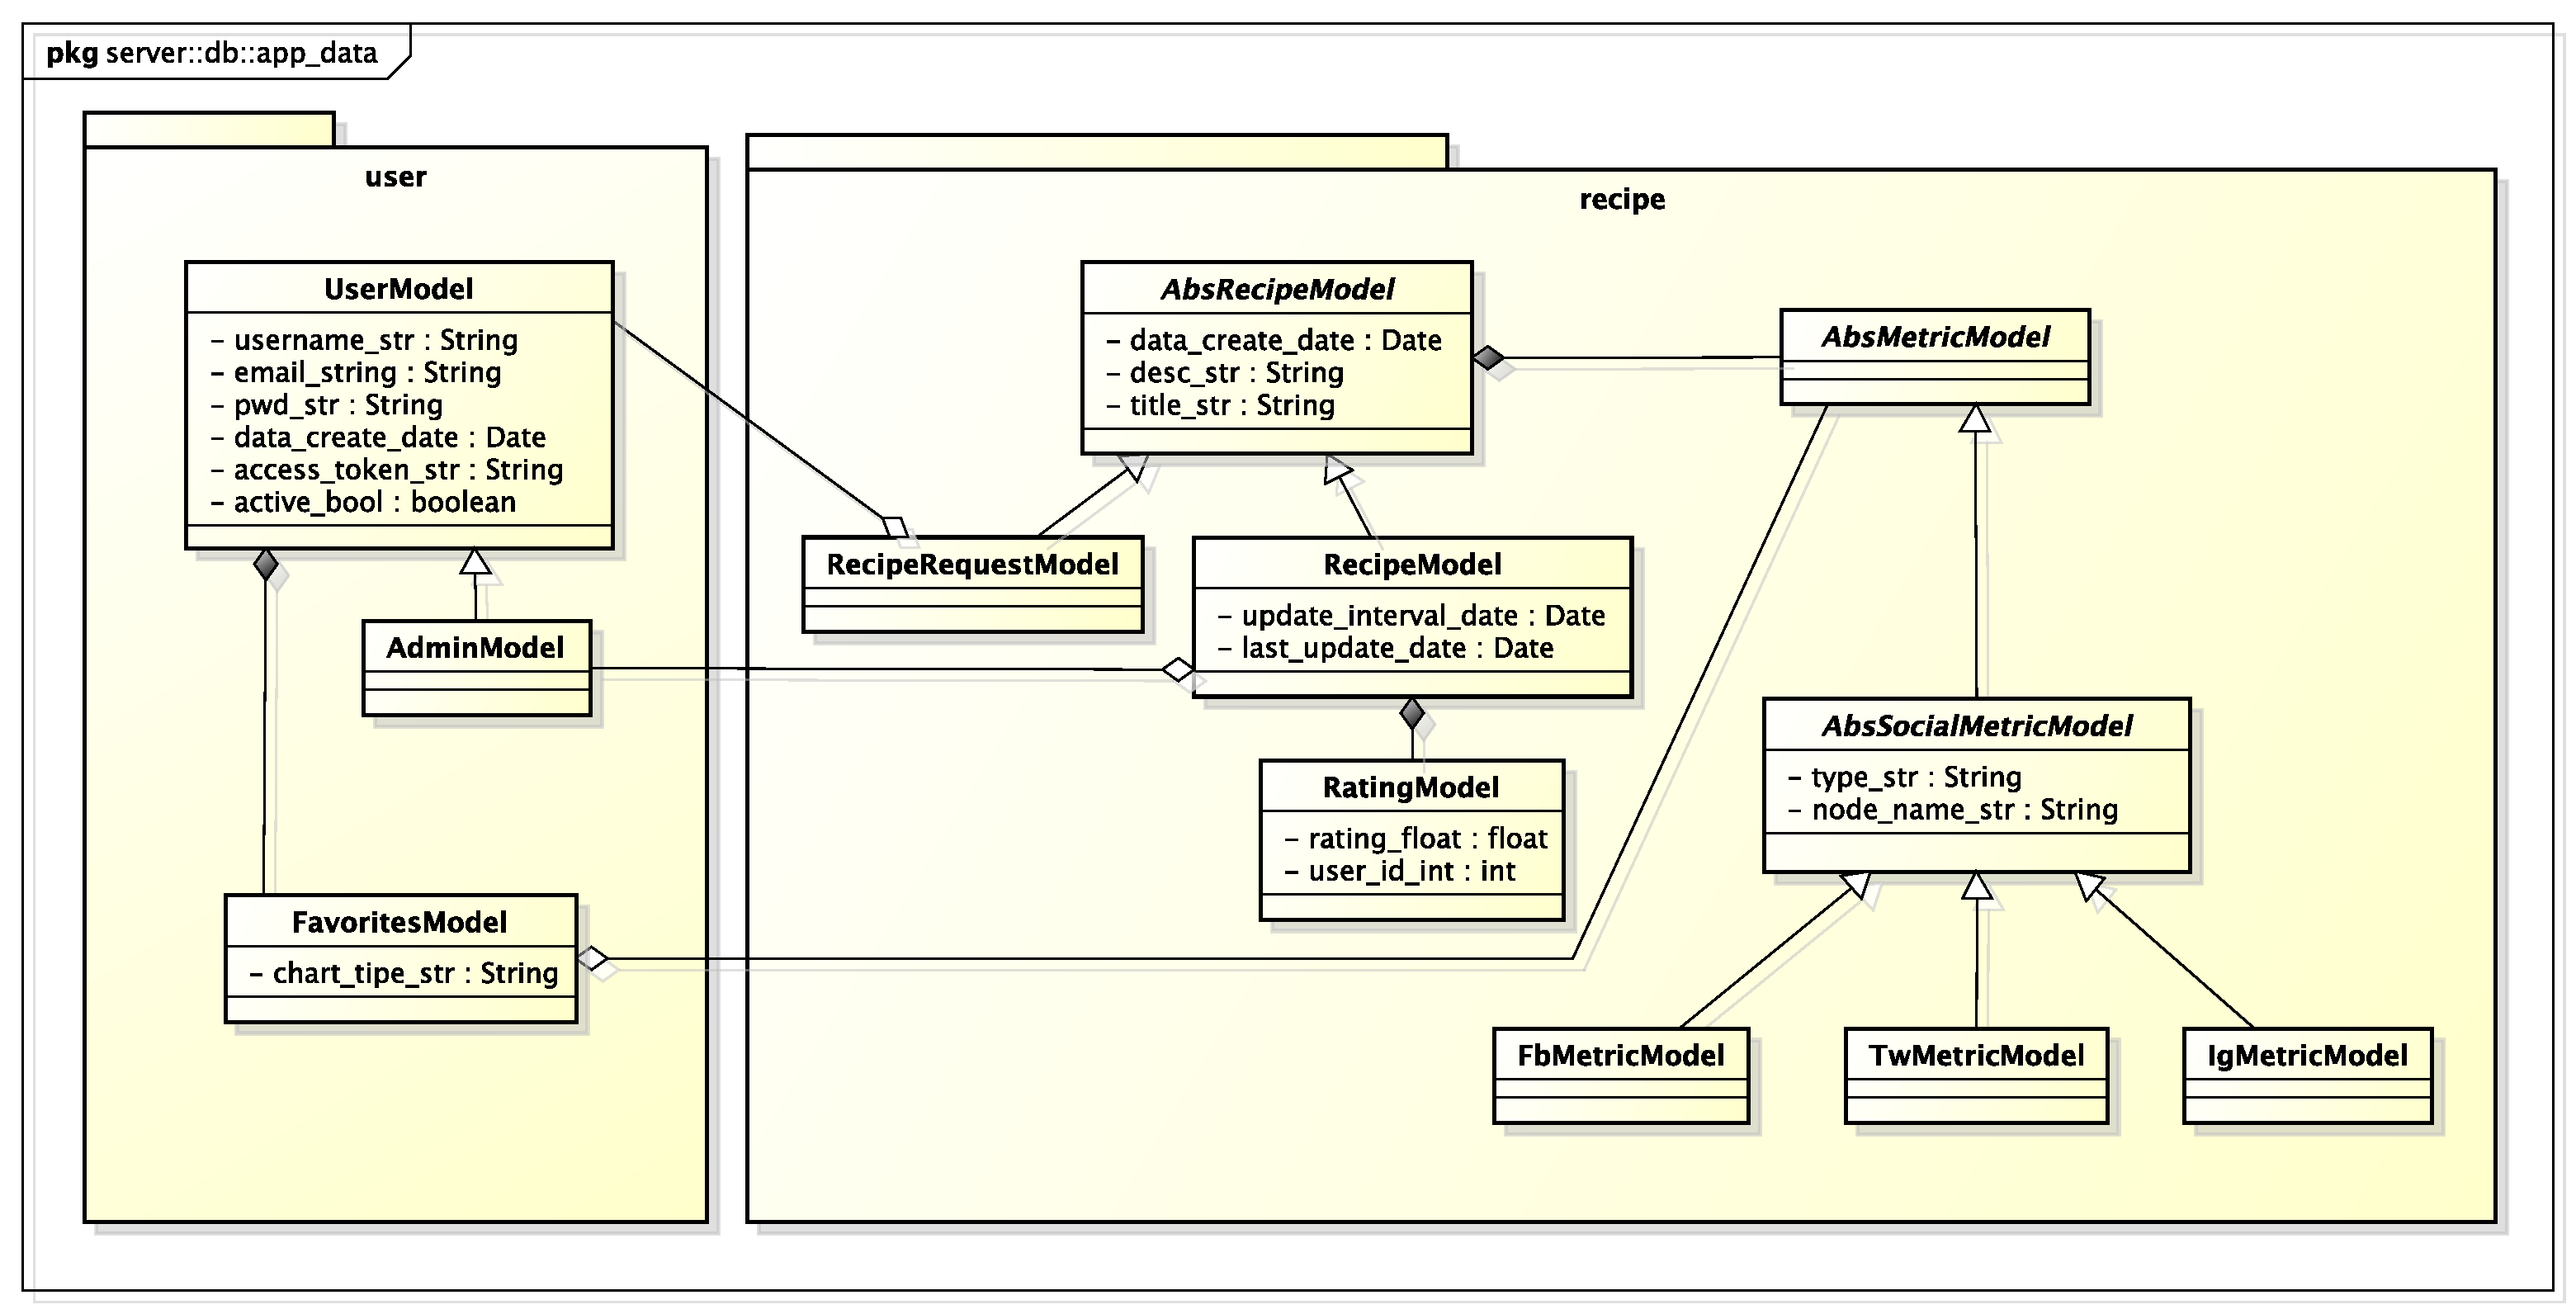
\includegraphics[scale=0.38]{./images/server/app_data.pdf}}
		\caption{Package - server::db::app\_data}
	\end{figure}


	\begin{itemize}
		\item \textbf{Descrizione}: è il package che contiene la definizione dei modelli degli utenti registrati e le loro preferenze. Contiene inoltre il modello delle Recipe che l'amministratore decide di creare;
		\item \textbf{Padre}: server::db
		\item \textbf{Package contenuti}
			\begin{itemize}
				\item server::db::app\_data::user
				\item server::db::app\_data::recipe
			\end{itemize}
	\end{itemize}
	% subsubsection bdsm_app_server_app_data [end]


\subsubsection{server::db::app\_data::user} % (fold)
\label{ssub:bdsm_app_server_app_data_user}

	\begin{itemize}
		\item \textbf{Descrizione}: è il package che contiene la definizione dei modelli degli utenti registrati e le loro preferenze;
		\item \textbf{Padre}: server::db::app\_data
		\item \textbf{Interazione con altri componenti}:
			\begin{itemize}
				\item server::db::app\_data::recipe
			\end{itemize}
	\end{itemize}
	% subsubsection bdsm_app_server_app_data_user [end]


	\paragraph{Classi} % (fold)

		\subparagraph{server::db::app\_data::user::UserModel} % (fold)
		\label{subp:server_db_app_data_user_user_model}
			\begin{figure}[htbp]
				\centering
				\centerline{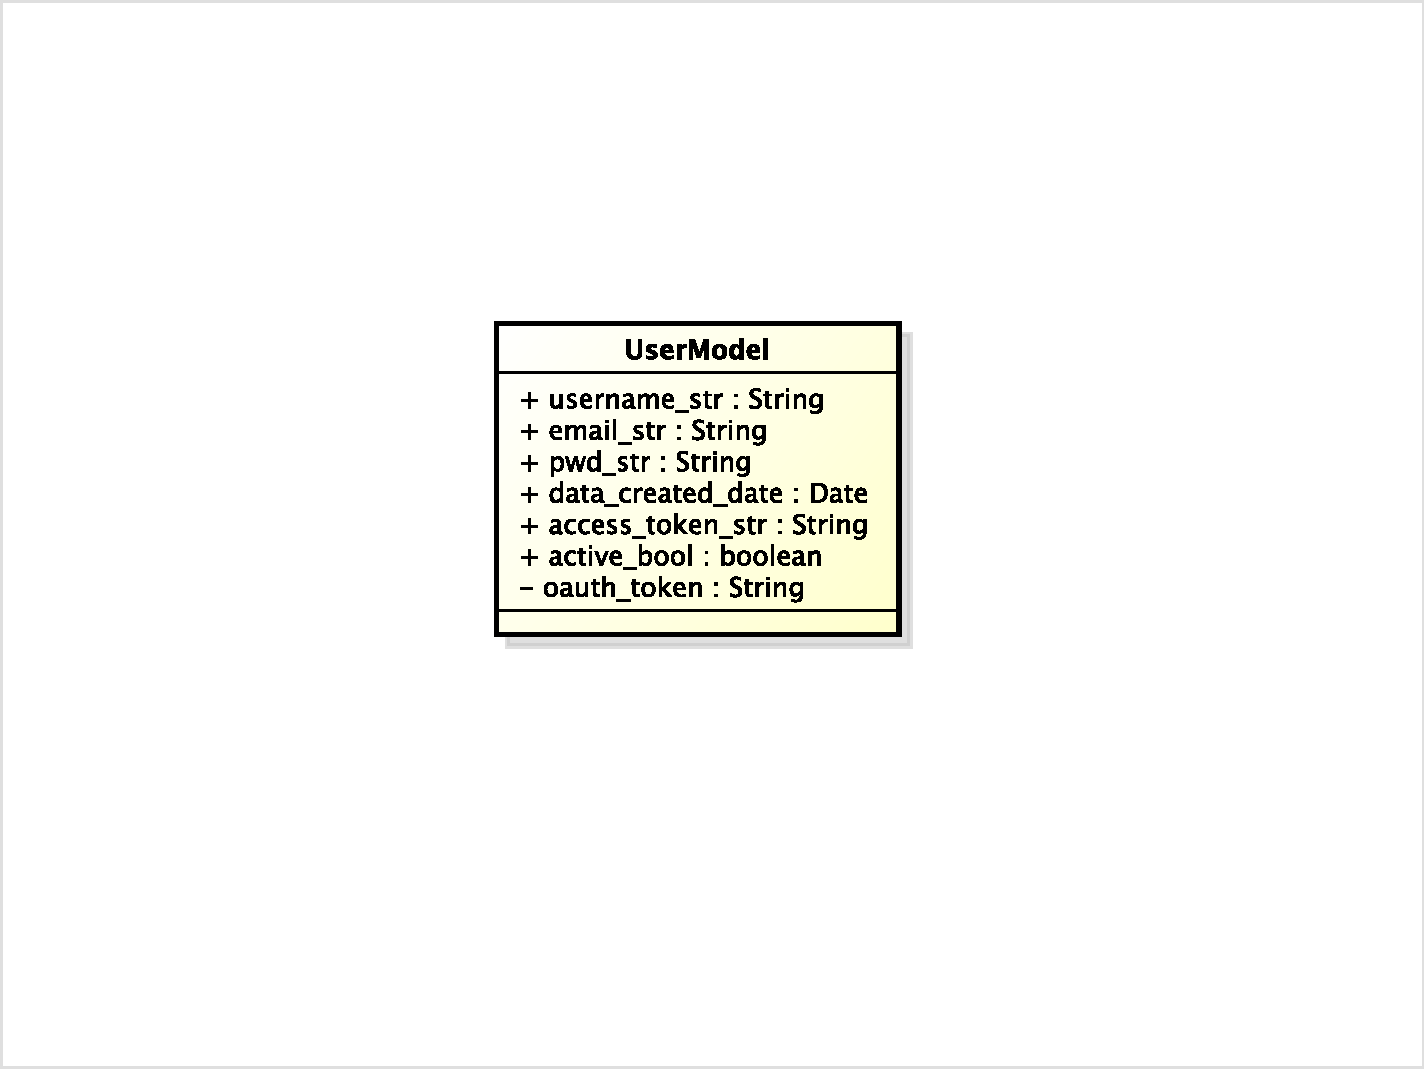
\includegraphics[scale=0.75]{./images/server/classes/db/user_model.pdf}}
				\caption{Classe - server::db::app\_data::user::UserModel}
			\end{figure}
			\begin{itemize}
				\item \textbf{Descrizione}: classe che definisce il modello dei dati degli utenti all'interno della base di dati;
				\item \textbf{Utilizzo}: la classe conterrà i metodi per la creazione, eliminazione, modifica degli account utente;
				\item \textbf{Relazioni con altre classi}:
					\begin{itemize}
						\item server::db::app\_data::user::FavouritesModel
						\item server::db:::app\_data::user::AdminModel
						\item server::db::app\_data::recipe::RecipeRequestModel
					\end{itemize}
				\item \textbf{Attributi}:
					\begin{itemize}
						\item \textcolor{forestgreen}{\texttt{+ username\_str : String}}
						\begin{description}
							\item \textbf{Descrizione}: username utente
						\end{description}
						\item \textcolor{forestgreen}{\texttt{+ email\_str : String}}
						\begin{description}
							\item \textbf{Descrizione}: email utente
						\end{description}
						\item \textcolor{forestgreen}{\texttt{+ pwd\_str : String}}
						\begin{description}
							\item \textbf{Descrizione}: password utente
						\end{description}
						\item \textcolor{forestgreen}{\texttt{+ data\_created\_date : Date}}
						\begin{description}
							\item \textbf{Descrizione}: data creazione account utente
						\end{description}
						\item \textcolor{forestgreen}{\texttt{+ access\_token\_str : String}}
						\begin{description}
							\item \textbf{Descrizione}: access token utente per i servizi rest
						\end{description}
						\item \textcolor{forestgreen}{\texttt{+ active\_bool : boolean}}
						\begin{description}
							\item \textbf{Descrizione}: utente attivo o disattivo
						\end{description}
					\end{itemize}
				\item \textbf{Metodi}: N/A
			\end{itemize}
		% subparagraph server_db_app_data_user_user_model [end]


		\subparagraph{server::db::app\_data::user::AdminModel} % (fold)
		\label{subp:server_db_app_data_user_admin_model}
			\begin{itemize}
				\item \textbf{Descrizione}: classe che definisce il modello dei dati degli utenti amministratori all'interno della base di dati;
				\item \textbf{Utilizzo}: la classe specializza l'utente amministratore. Viene implementata con dei metodi per l'aggiunta la modifica e la rimozione;
				\item \textbf{Classi ereditate}: server::db::app\_data::user::UserModel;
				\item \textbf{Relazioni con altre classi}:
					\begin{itemize}
						\item server::db::app\_data::recipe::RecipeModel
					\end{itemize}
				\item \textbf{Attributi}: N/A
				\item \textbf{Metodi}: N/A
			\end{itemize}
		% subparagraph server_db_app_data_user_admin_model [end]


		\subparagraph{server::db::app\_data::user::FavouritesModel} % (fold)
		\label{subp:server_db_app_data_user_favorites}
			\begin{figure}[htbp]
				\centering
				\centerline{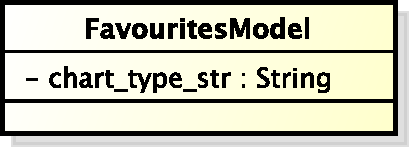
\includegraphics[scale=0.75]{./images/server/classes/db/favourites_model.pdf}}
				\caption{Classe - server::db::app\_data::user::FavouritesModel}
			\end{figure}
			\begin{itemize}
				\item \textbf{Descrizione}: classe che definisce il modello dei dati relativo ai preferiti dell'utente;
				\item \textbf{Utilizzo}: la classe  permette all'utente di aggiungere dei modelli di view nei preferiti. Contiene metodi per l'inserimento e rimozione di preferiti;
				\item \textbf{Relazioni con altre classi}:
					\begin{itemize}
						\item server::db::app\_data::recipe::AbsMetricModel
					\end{itemize}
				\item \textbf{Attributi}:
					\begin{itemize}
						\item \textcolor{forestgreen}{\texttt{chart\_type\_str : String}}
						\begin{description}
							\item \textbf{Descrizione}: tipo di grafico scelto dall'utente e salvato nei preferiti
						\end{description}
					\end{itemize}
				\item \textbf{Metodi}: N/A
			\end{itemize}
		% subparagraph server_db_app_data_user_favorites [end]


\subsubsection{server::db::app\_data::recipe} % (fold)
\label{ssub:bdsm_app_server_app_data_recipe}

	\begin{itemize}
		\item \textbf{Descrizione}: è il package che contiene la definizione dei modelli delle Recipe che l'amministratore decide di creare;
		\item \textbf{Padre}: server::db::app\_data
		\item \textbf{Interazione con altri componenti}:
			\begin{itemize}
				\item server::db::app\_data::user
			\end{itemize}
	\end{itemize}
	% subsubsection bdsm_app_server_app_data_recipe [end]


	\paragraph{Classi} % (fold)

		\subparagraph{server::db::app\_data::recipe::AbsRecipeModel} % (fold)
		\label{subp:server_db_app_data_recipe_absrecipemodel}
			\begin{figure}[htbp]
				\centering
				\centerline{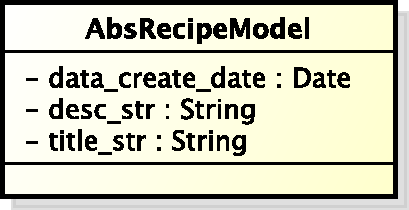
\includegraphics[scale=0.75]{./images/server/classes/db/abs_recipe_model.pdf}}
				\caption{Classe - server::db::app\_data::recipe::AbsRecipeModel}
			\end{figure}
			\begin{itemize}
				\item \textbf{Descrizione}: classe astratta che rappresenta un modello comune per Recipe e richiesta di aggiunta Recipe;
				\item \textbf{Utilizzo}: la classe mantiene l'estensibilità per eventuali nuovi tipi di Recipe;
				\item \textbf{Relazioni con altre classi}:
					\begin{itemize}
						\item server::db::app\_data::recipe::RecipeModel
						\item server::db::app\_data::recipe::RecipeRequestModel
						\item server::db::app\_data::recipe::AbsMetricModel
					\end{itemize}
				\item \textbf{Attributi}:
					\begin{itemize}
						\item \textcolor{forestgreen}{\texttt{data\_create\_date : Date}}
						\begin{description}
							\item \textbf{Descrizione}: data creazione recipe
						\end{description}
						\item \textcolor{forestgreen}{\texttt{desc\_str : String}}
						\begin{description}
							\item \textbf{Descrizione}: descrizione dettagliata recipe
						\end{description}
						\item \textcolor{forestgreen}{\texttt{title\_str : String}}
						\begin{description}
							\item \textbf{Descrizione}: titolo recipe
						\end{description}
					\end{itemize}
				\item \textbf{Metodi}: N/A
			\end{itemize}
		% subparagraph server_db_app_data_recipe_absrecipemodel [end]


		\subparagraph{server::db::app\_data::recipe::RecipeRequestModel} % (fold)
		\label{subp:server_db_app_data_recipe_reciperequestmodel}
			\begin{itemize}
				\item \textbf{Descrizione}: classe che definisce il modello dei dati per la richiesta di aggiunta Recipe;
				\item \textbf{Utilizzo}: la classe specializza la richiesta identificandone l'utente;
				\item \textbf{Classi ereditate}: server::db::app\_data::recipe::AbsRecipeModel
				\item \textbf{Attributi}: N/A
				\item \textbf{Metodi}: N/A
			\end{itemize}
		% subparagraph server_db_app_data_recipe_reciperequestmodel [end]


		\subparagraph{server::db::app\_data::recipe::RecipeModel} % (fold)
		\label{subp:server_db_app_data_recipe_recipemodel}
			\begin{figure}[htbp]
				\centering
				\centerline{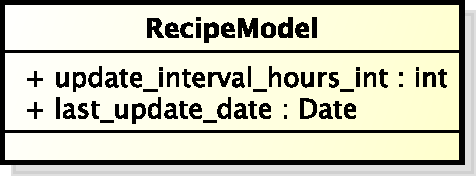
\includegraphics[scale=0.75]{./images/server/classes/db/recipe_model.pdf}}
				\caption{Classe - server::db::app\_data::recipe::RecipeModel}
			\end{figure}
			\begin{itemize}
				\item \textbf{Descrizione}: classe che definisce il modello dei dati realtivo ad una Recipe;
				\item \textbf{Utilizzo}: la classe specializza la ricetta. Vengono forniti i campi dati per il possibile incremento temporale dei dati;
				\item \textbf{Classi ereditate}: server::db::app\_data::recipe::AbsRecipeModel
				\item \textbf{Relazioni con altre classi}:
					\begin{itemize}
						\item server::db::app\_data::recipe::RatingModel
					\end{itemize}
				\item \textbf{Attributi}:
					\begin{itemize}
						\item \textcolor{forestgreen}{\texttt{+ update\_interval\_hours\_int : int}}
						\begin{description}
							\item \textbf{Descrizione}: intervallo di tempo schedulazione recipe
						\end{description}
						\item \textcolor{forestgreen}{\texttt{+ last\_update\_date : Date}}
						\begin{description}
							\item \textbf{Descrizione}: data ultimo avvio miner recipe
						\end{description}
					\end{itemize}
				\item \textbf{Metodi}: N/A
			\end{itemize}
		% subparagraph server_db_app_data_recipe_recipemodel [end]

		\subparagraph{server::db::app\_data::recipe::RatingModel} % (fold)
		\label{subp:server_db_app_data_recipe_recipemodel}
			\begin{figure}[htbp]
				\centering
				\centerline{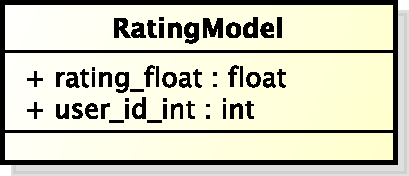
\includegraphics[scale=0.75]{./images/server/classes/db/rating_model.pdf}}
				\caption{Classe - server::db::app\_data::recipe::RatingModel}
			\end{figure}
			\begin{itemize}
				\item \textbf{Descrizione}: classe che rappresenta il modello del rating di una Recipe;
				\item \textbf{Utilizzo}: viene utilizzata per risalire al voto di ogni utente per una determinata Recipe;
				\item \textbf{Attributi}:
					\begin{itemize}
						\item \textcolor{forestgreen}{\texttt{+ rating\_float : float}}
						\begin{description}
							\item \textbf{Descrizione}: punteggio gradimento recipe utente
						\end{description}
						\item \textcolor{forestgreen}{\texttt{+ user\_id\_int : int}}
					\end{itemize}
					\begin{description}
							\item \textbf{Descrizione}: identificativo utente votante
						\end{description}
				\item \textbf{Metodi}: N/A
			\end{itemize}
		% subparagraph server_db_app_data_recipe_recipemodel [end]


		\subparagraph{server::db::app\_data::recipe::AbsMetricModel} % (fold)
		\label{subp:server_db_app_data_recipe_absmetricmodel}
			\begin{itemize}
				\item \textbf{Descrizione}: classe che definisce il modello dei dati di una metrica contenuta in una Ricetta;
				\item \textbf{Utilizzo}: la classe ha il compito di inglobare tutte le sotto-metriche e non solo quelle derivate dai social media;
				\item \textbf{Relazioni con altre classi}:
					\begin{itemize}
						\item server::db::app\_data::recipe::AbsSocialMetricModel
					\end{itemize}
				\item \textbf{Attributi}: N/A
				\item \textbf{Metodi}: N/A
			\end{itemize}
		% subparagraph server_db_app_data_recipe_absmetricmodel [end]


		\subparagraph{server::db::app\_data::recipe::AbsSocialMetricModel} % (fold)
		\label{subp:server_db_app_data_recipe_abssocialmetricmodel}
			\begin{figure}[htbp]
				\centering
				\centerline{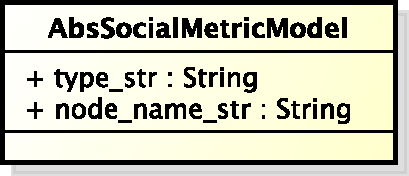
\includegraphics[scale=0.75]{./images/server/classes/db/abs_social_metric_model.pdf}}
				\caption{Classe - server::db::app\_data::recipe::AbsSocialMetricModel}
			\end{figure}
			\begin{itemize}
				\item \textbf{Descrizione}: classe che definisce il modello dei dati delle metriche relative ai social media;
				\item \textbf{Utilizzo}: la classe ha il compito di raggruppare i social media da rappresentare e identificarli univocamente;
				\item \textbf{Classi ereditate}: server::db::app\_data::recipe::AbsMetricModel
				\item \textbf{Relazioni con altre classi}:
					\begin{itemize}
						\item server::db::app\_data::recipe::FbMetricModel
						\item server::db::app\_data::recipe::IgMetricModel
						\item server::db::app\_data::recipe::TwMetricModel
					\end{itemize}
				\item \textbf{Attributi}:
					\begin{itemize}
						\item \textcolor{forestgreen}{\texttt{+ type\_str : String}}
						\begin{description}
							\item \textbf{Descrizione}: tipo di metrica
						\end{description}
						\item \textcolor{forestgreen}{\texttt{+ node\_name\_str : String}}
						\begin{description}
							\item \textbf{Descrizione}: nome categoria metrica
						\end{description}
					\end{itemize}
				\item \textbf{Metodi}: N/A
			\end{itemize}
		% subparagraph server_db_app_data_recipe_abssocialmetricmodel [end]


		\subparagraph{server::db::app\_data::recipe::FbMetricModel} % (fold)
		\label{subp:server_db_app_data_recipe_fbmetricmodel}
			\begin{itemize}
				\item \textbf{Descrizione}: classe che definisce il modello dei dati delle metriche relative a Facebook;
				\item \textbf{Utilizzo}: la classe ha il compito di identificare univocamente l'id della pagina o l'id dell'evento da analizzare. La classe fornisce metodi per l'aggiunta e la rimozione ricorsiva in caso di cancellazione;
				\item \textbf{Classi ereditate}: server::db::app\_data::recipe::AbsSocialMetricModel;
				\item \textbf{Attributi}: N/A
				\item \textbf{Metodi}: N/A
			\end{itemize}
		% subparagraph server_db_app_data_recipe_fbmetricmodel [end]


		\subparagraph{server::db::app\_data::recipe::IgMetricModel} % (fold)
		\label{subp:server_db_app_data_recipe_igmetricmodel}
			\begin{itemize}
				\item \textbf{Descrizione}: classe che definisce il modello dei dati delle metriche relative a Instagram;
				\item \textbf{Utilizzo}: la classe ha il compito di identificare univocamente l'id della pagina o l'hashtag da analizzare. La classe fornisce metodi per l'aggiunta e la rimozione ricorsiva in caso di cancellazione;
				\item \textbf{Classi ereditate}: server::db::app\_data::recipe::AbsSocialMetricModel;
				\item \textbf{Attributi}: N/A
				\item \textbf{Metodi}: N/A
			\end{itemize}
		% subparagraph server_db_app_data_recipe_igmetricmodel [end]


		\subparagraph{server::db::app\_data::recipe::TwMetricModel} % (fold)
		\label{subp:server_db_app_data_recipe_twmetricmodel}
			\begin{itemize}
				\item \textbf{Descrizione}: classe che definisce il modello dei dati delle metriche relative a Twitter;
				\item \textbf{Utilizzo}: la classe ha il compito di identificare univocamente l'id della pagina o l'hashtag da analizzare. La classe fornisce metodi per l'aggiunta e la rimozione ricorsiva in caso di cancellazione;
				\item \textbf{Classi ereditate}: server::db::app\_data::recipe::AbsSocialMetricModel;
				\item \textbf{Attributi}: N/A
				\item \textbf{Metodi}: N/A
			\end{itemize}
		% subparagraph server_db_app_data_recipe_twmetricmodel [end]
